% %%%%%%%%%%%%%%%%%%%%%%%%%%%%%%%%%%%%%%%%%%%%%%%%%%%%%%%%%%%%%%%%%%%%%%%%%%%%%%%%%%%%%%%%%%%%%%%%%%%%
% %%%%%%%%%%%%%%%%%%%%%%%%%%%%%%%%%%%%%%%%%%%%%%%%%%%%%%%%%%%%%%%%%%%%%%%%%%%%%%%%%%%%%%%%%%%%%%%%%%%%
% ZEROWASTE
% %%%%%%%%%%%%%%%%%%%%%%%%%%%%%%%%%%%%%%%%%%%%%%%%%%%%%%%%%%%%%%%%%%%%%%%%%%%%%%%%%%%%%%%%%%%%%%%%%%%%
% %%%%%%%%%%%%%%%%%%%%%%%%%%%%%%%%%%%%%%%%%%%%%%%%%%%%%%%%%%%%%%%%%%%%%%%%%%%%%%%%%%%%%%%%%%%%%%%%%%%%

\graphicspath{{./\figurefolder/6ZeroWaste/}}
\setlist{topsep=1.5em, itemsep=0.5em}

% ----------------------------------------------------------------------------------------------------
% 0. Front Matter
% ----------------------------------------------------------------------------------------------------
\chapter{Coopearative Robotic Disassembly and Reuse of a Timber Frame Structure}\label{chap:6_ZeroWaste}

\thispagestyle{empty}

\vfill 
\section*{\normalsize\textmd{This chapter is based on the following publication:}}
    \vspace{-0.3cm}
    \textbf{Bruun, E. P. G.}, Adriaenssens, S., Besler, E., \& Parascho, S. (2024). ZeroWaste: Disassembly and Reuse of a Timber Frame Structure using Cooperating Robots. Construction Robotics. (Accepted)

    % \textbf{Bruun, E. P. G.}, Adriaenssens, S., Besler, E., \& Parascho, S. (2022). ZeroWaste: Towards Computing Cooperative Robotic Sequences for the Disassembly and Reuse of Timber Frame Structures. Proceedings of the 42nd Annual Conference of the Association for Computer Aided Design in Architecture, 586–597. http://arks.princeton.edu/ark:/88435/pr1wp9t657

\section*{\normalsize\textmd{Contributor roles in publication:}}
    \vspace{-0.3cm}\noindent
    - Bruun: Conceptualization, Methodology, Software, Validation, Investigation, Writing (Original Draft), Writing (Review and Editing), Visualization\\
    - Adriaenssens: Writing (Review and Editing), Supervision, Funding Acquisition \\
    - Besler: Conceptualization, Resources, Writing (Review and Editing), Funding Acquisition \\
    - Parascho: Conceptualization, Resources, Writing (Review and Editing), Supervision, Funding Acquisition \\
    
    
% \section*{\normalsize\textmd{Acknowledgements:}}
%     \vspace{-0.3cm}
%     This research was partially developed with input from the following people at the early ideation stages of the project: Chris Myefski, Chase Galis, and Ian Ting.


    \newpage
    \begin{figure}[ht]
        \centering
        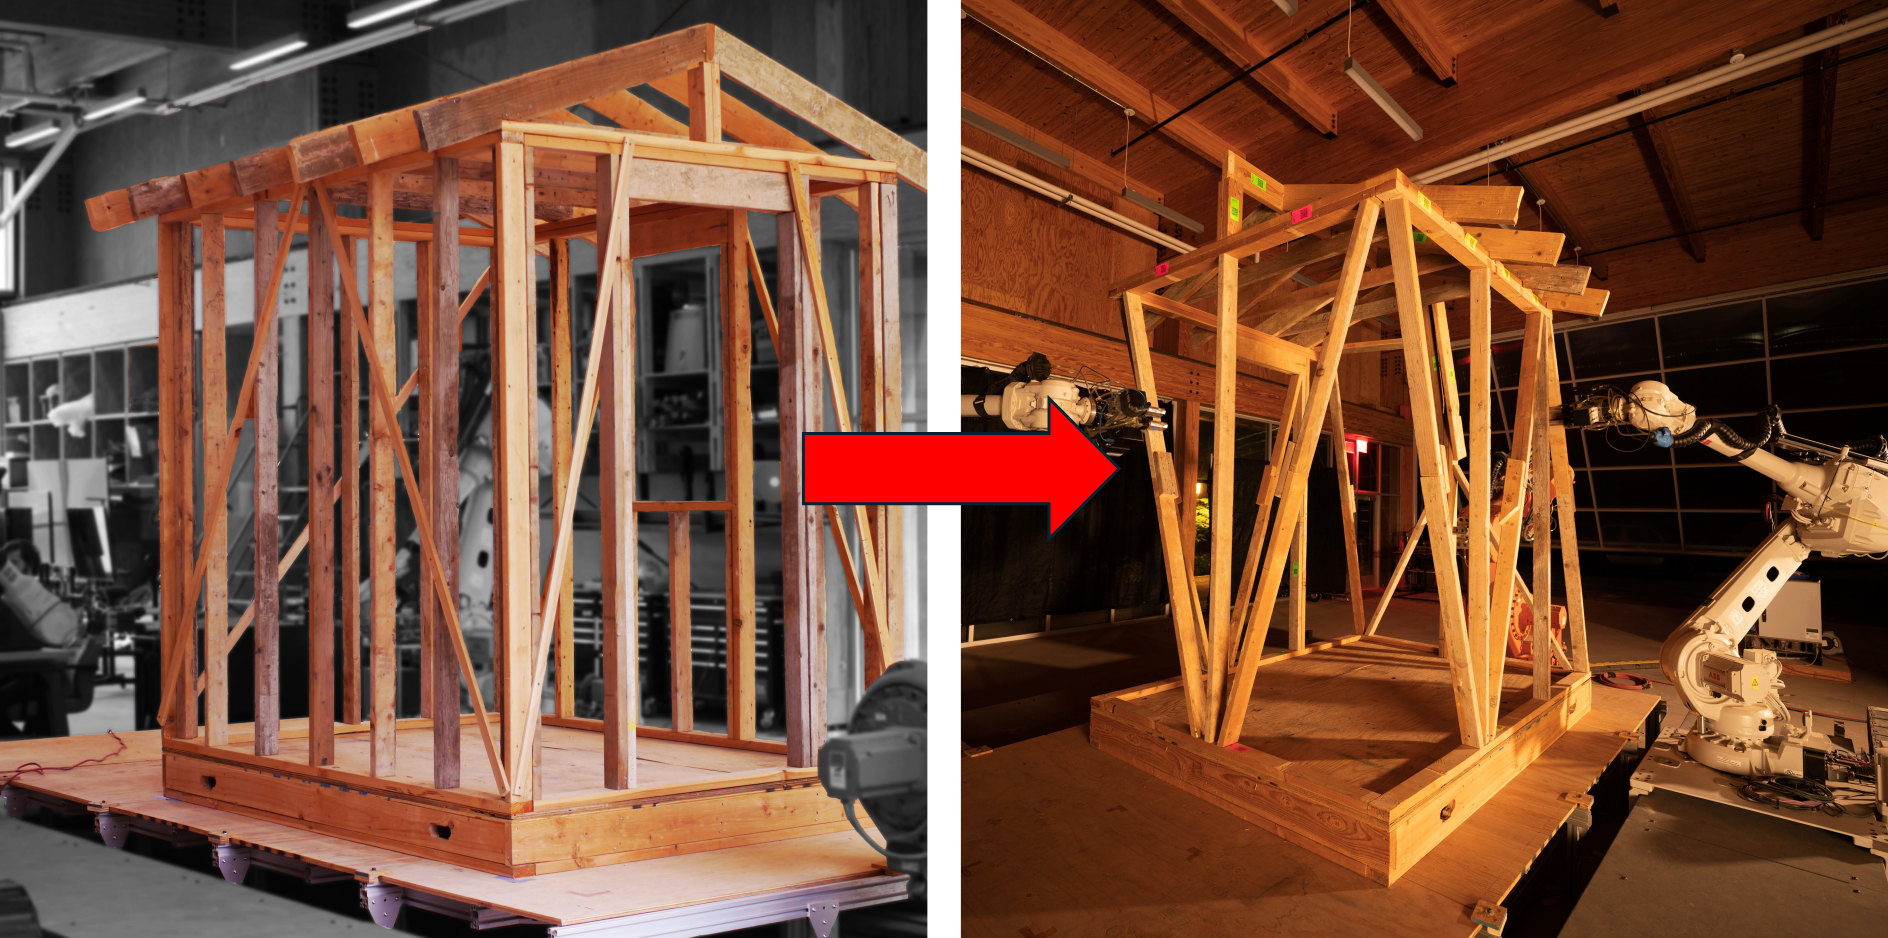
\includegraphics [trim={0cm 0cm 0cm 0cm},clip,width=0.85\textwidth]{_cover_structure}
        \caption{An existing timber structure is disassembled and reassembled into a new configuration with a team of cooperating robots.}
        \label{fig:chapter6_title}
    \end{figure}%

\section*{Abstract}
    This chapter presents the results of the ZeroWaste project, showcasing how circular economy principles are realized through cooperative robotic fabrication methods. A pavilion-scale conventional stick frame prototype structure is initially constructed (as shown on the left in \cref{fig:chapter6_title}). Precise geometric data is then obtained using a robotic cell equipped with three large-scale robotic arms and 3D cameras, facilitating planning of robotic processes. A novel topological representation, the support hierarchy graph, is developed to generate fabrication sequences, assessed for robotic execution and structural feasibility. Leveraging the cooperative robotic setup, disassembly sequences are planned without external scaffolding, as the robots are used to provide temporary support. Three physical fabrication phases validate the computational and robotic workflow: Phase 1 involves small-scale disassembly, Phase 2 expands to full wall disassembly with minor reassembly, and Phase 3 disassembles remaining members while concurrently reassembling them to create a stiffer lattice structure. These fabrication phases result in a modified structural configuration (as shown on the right in \cref{fig:chapter6_title}) that demonstrates the potential of existing buildings to be used as reservoirs of reusable materials through the implementation of scaffold-free cooperative robotic disassembly and reassembly methods.


% ----------------------------------------------------------------------------------------------------
% 1. Introduction
% ----------------------------------------------------------------------------------------------------
\clearpage
\section{Introduction}
    The Architecture, Engineering, Construction (AEC) industry has a significant negative impact on the environment due to its material and energy-intensive manufacturing and construction processes \citep{international_energy_agency_2018_2018} and the high embodied carbon content of structural systems \citep{kaethner_embodied_2012, fang_reducing_2023}. For example, buildings and construction activities accounted for 36\% of global energy-usage and of 37\% of global CO2 emissions in 2020 \citep{united_nations_global_2021}. This impact is further exacerbated by the increasing waste generated by construction and demolition (C\&D) processes \citep{us_epa_construction_2018, us_epa_construction_2020}, which were estimated to account for up to 30\% of total waste produced globally in the 1990s \citep{purchase_circular_2022, fishbein_building_1998}.
    
    To illustrate this worsening trend, in the mid-1990s in the United States, construction and demolition (C\&D) activities were responsible for generating an estimated 100-135 million tons of waste, of which approximately 35-45\% found its way to landfills \citep{mills_cost-effective_1999, us_epa_characterization_1998}. This C\&D waste accounted for 29\% of the total landfill volumes at that time \citep{lu_framework_2011}. However, by 2018, the volume of waste from C\&D activities had surged to 600 million tons, with 144 million tons or 24\% of this waste ending up in landfills \citep{us_epa_advancing_2020}. Thus, approximately half of landfill volumes in 2018 were associated with C\&D activities, with the remaining municipal solid waste contributing 146 million tons \citep{us_epa_advancing_2020}. This trend is especially concerning when considering the substantial construction needs of the coming century. Aging infrastructure must be replaced while accommodating the requirements of a growing and rapidly urbanizing global population \citep{ritchie_urbanization_2018}.

    Reducing the construction industry's material usage and waste generation involves harnessing technological advancements such as robotics and automation to boost productivity and efficiency of construction processes. However, this is only one part of the solution, as addressing waste begins at the design phase, where strategic planning can significantly reduce material usage and waste generation throughout the project life cycle. Research indicates that a notable portion of construction waste stems from inadequate waste reduction measures early in the design stages, particularly in planning for building decommissioning \citep{osmani_architects_2008}. With demolition accounting for over 90\% of construction and demolition (C\&D) debris generation \citep{us_epa_advancing_2020}, the industry faces a pressing need for transformation. Therefore, adopting a design paradigm centered on deconstruction and material reuse aligns with the principles of a circular economy \citep{geissdoerfer_circular_2017}, and presents a possible solution to the industry's waste challenges.

\subsection{Chapter Organization}
    The chapter is structured into several key sections to comprehensively present the research. First, in \Cref{sec:2_lit}, a literature review is presented, covering topics such as circular economy design frameworks and robotic fabrication within the context of material circularity. An overview of the ZeroWaste project, which forms the basis of this chapter, is also provided specifically describing how the project addresses circular economy and robotic fabrication through its research objectives. Following this, in \Cref{sec:3_experimental_setup}, the experimental setup is outlined, describing the physical robotic fabrication cell and the experimental prototype that is built and then experimented on in the three subsequent project phases. In \Cref{sec:4_experimental_methods}, the workflow and methods are detailed, focusing on the computational methods developed for various aspects of the project. This includes the use of robot-mounted 3D cameras to gather geometric information about the as-built conditions of the structure, the development of the topological support hierarchy representation, and the methods used to generate robotic fabrication sequences and assess their feasibility. In \Cref{sec:5_results}, the results of implementing the computational methods described in the previous section to plan and then execute three different disassembly and reassembly robotic fabrication tasks on the prototype structure are presented and discussed. Finally, in \Cref{sec:6_conclusion}, the chapter concludes with a summary of the main results and discussions from the fabrication tasks performed on the prototype structure, and suggesting ideas for future work stemming from limitations of the current work.


% ----------------------------------------------------------------------------------------------------
% 2. Literature Review
% ----------------------------------------------------------------------------------------------------
\section{Literature Review} \label{sec:2_lit}

\subsection{Circular Economy Design Frameworks} \label{sec:2a_circular}
    The construction industry is actively moving away from the traditional linear single-use material flow model. To support this transition, there has been a focus on developing models for quantifying the environmental benefits of material circularity and the potential for reusing existing building stock, as evidenced in works such as \cite{cottafava_circularity_2021, eberhardt_circular_2021}. In parallel, novel frameworks have emerged that break down the concept of circularity into distinct principles relating to material and energy flows. An illustrative framework is the ``narrow, slow, close, and regenerate'' framework outlined in \cite{konietzko_circular_2020, cetin_circular_2021}, which serves as the basis for a recent book on shifting to the circular built environment while leveraging modern digital technologies \citep{de_wolf_circular_2023}.
    
    Specifically, the ``slow'' principle, which focuses on extending the lifespan of products and components, encompasses a range of circular product design and business strategies that are applicable to the building industry \citep{bocken_product_2016}. One such strategy, known as ``design for dis- and reassembly,'' is demonstrated by a growing body of research that highlihgts practical implementation of design and optimization strategies for the disassembly, reuse, and reconfiguration of discrete element structures. This includes examples applied to a variety of structural systems like planar trusses \citep{brutting_design_2019, naboni_design_2021}, space frames \citep{brutting_design_2021, bruun_structural_2022}, moment frames \citep{brutting_optimum_2020}, reciprocal frames \citep{glath_thinking_2022, zahiri_sequential_2023}.

\subsection{Robotic Fabrication and Material Circularity} \label{sec:2b_robs}
    The construction industry, despite its potential to benefit from technological advancements that enhance efficiency, has been slow in embracing automation technology and realizing productivity gains in comparison to other sectors, as observed over the last five decades \citep{barbosa_reinventing_2017}. Nonetheless, an opportunity still exists to leverage modern technological innovations, with a particular focus on the use of robots to improve the productivity of construction \citep{the_business_research_company_global_2023}, particularly when applied to the construction of geometrically complex and materially efficient bespoke structures \citep{garcia_de_soto_productivity_2018}.
    
    In the initial phase of introducing robots to the construction industry during the 1980s, the primary focus was on utilizing single robots to automate individual human tasks \citep{bock_construction_2007, bock_construction_2016}. In recent years, however, researchers have shifted their focus from task-specific automation towards am approach that integrates robots into a broader construction context, using more complex robotic setups for collaborative and adaptive construction processes to expand the possibilities of what can be designed and built \citep{gramazio_digital_2008,parascho_construction_2023}. This shift involves leveraging the unique capabilities of robots, such as their precision in repetitive movement, accurate spatial positioning of components, and ability to perform long-duration tasks. For instance, the adoption of a cooperative robotic fabrication framework, first demonstrated in \cite{parascho_cooperative_2017}, has emerged as a promising avenue, demonstrating the potential to enhance both fabrication complexity and the degree of automation \citep{bruun_three_2021, mesnil_flexible_2023}. Cooperative robotic fabrication, a specialized form of robotic manufacturing, entails synchronized robotic agents working together to achieve greater system utility and unique outcomes that would be unattainable with independent robot operation \citep{cao_cooperative_1997}. This stands in contrast to collaborative robotic processes, where human operators work alongside robotic setups, occurring in either a cooperative robotic \citep{bruun_humanrobot_2020} or non-cooperative robotic setting \citep{weckenborg_balancing_2020}.
    
    The benefits of utilizing multiple robots collaborating go beyond just improving production efficiency. Cooperative robotic fabrication projects have explicitly demonstrated principles of circular economy and material circularity. A recent review titled ``Cooperative Robotic Fabrication for a Circular Economy'' by \cite{bruun_cooperative_2024} provides a comprehensive overview of the general applications of cooperative robotic fabrication in the construction industry. The review further delves into these applications within the specific context of material reuse and reduction as integral components of a circular economy strategy. Examples of material reduction include minimizing the need for scaffolding during masonry \citep{parascho_robotic_2020, parascho_lightvault_2021, han_concept_2020} and steel \citep{parascho_cooperative_2017,parascho_computational_2018} structure construction through robot-assisted temporary support. Additionally, designing a timber space frame structures from the outset to be (dis)assembled in a scaffold-free manner with a cooperating team of robots as first demonstrated in \citep{bruun_structural_2022}.

    % \citep{parascho_robotic_2020, parascho_lightvault_2021, han_concept_2020, bruun_automating_2023}


\subsection{The ZeroWaste Project} \label{sec:2c_project}
    This chapter presents a comprehensive exploration of the ZeroWaste project, extending the research documented in recent publications \citep{bruun_cooperative_2024, bruun_zerowaste_2022}. It serves as a practical demonstrator and a pivotal link between the existing body of research in the field of circular economy (as outlined in \Cref{sec:2a_circular}) and the implementation of robotic automation technology in the construction industry (as outlined in \Cref{sec:2b_robs}).
    
    The research is conducted on a prefabricated timber prototype, which is meant to represent a generic unknown existing structure built according to the common North American stick frame construction practices. This choice is based on the prevalence of this building type coupled with the frequency that timber buildings are disposed of at the end their lives, as noted in previous studies \citep{obrien_life_2006, diyamandoglu_deconstruction_2015}. Notably, of the 40.8 million tons of wood construction debris generated in 2018 in the US, 72\% of this total is sent to landfills, where 92\% of this amount is attributed to demolition processes \citep{us_epa_advancing_2020}. To address this linear material flow, reimagining timber buildings as material depots is proposed, recognizing their potential as reservoirs of valuable resources in the context of a circular economy \citep{zimmann_circular_2016}. This shift prioritizes the upstream flow of materials on construction sites, reducing reliance on upstream virgin materials and downstream recycling and waste industries \citep{garcia_material_2021}. In addition, the aim is to perform all processes in a scaffold-free manner to reduce the materials typically required to provide support during assembly and disassembly.


    \subsubsection{Research Objectives}
        The ZeroWaste project is situated at the intersection of two key research areas: (1) circular economy and (2) robotic fabrication. The project aims to achieve various objectives that highlight the possibilities and benefits of combining these two research domains.
        
        The objectives related to circular economy principles are the following:
        \begin{enumerate}
            \item \textbf{Physical Implementation Study:} Demonstrate how existing timber buildings can serve as reservoirs of reusable materials.
            \item \textbf{Material Reuse:} Disassemble and reassemble portions of an existing prototype structure, demonstrating the potential for creating new configurations from previously used materials.
        \end{enumerate}
        
        The objectives related to robotic fabrication are the following:
        \begin{enumerate}
            \item \textbf{Cooperative Fabrication:} Harness the capabilities of a cooperative robotic setup, consisting of three large-scale robotic arms, working in a coordinated manner to improve the fabrication utility of the setup.
            \item \textbf{Fabrication Sequences:} Calculate feasible cooperative robotic assembly and disassembly sequences when considering constraints related to robotic reachability and structural stability.
            \item \textbf{Scaffold-free Construction:} Execute the fabrication sequences without the need for external temporary scaffolding, utilizing the robots themselves as passive structural supports.
            \item \textbf{Member Localization:} Utilize robot-mounted 3D cameras to generate geometrically precise as-built digital models of the existing timber prototype structure.
        \end{enumerate}
        
        The significance of these objectives extends beyond the specific structural prototype under study. They offer a versatile framework applicable to a wide range of timber structures and discrete element topologies. The ZeroWaste project serves as a compelling illustration of how circular economy principles can be integrated into construction practices, and it highlights the potential for modern robotic fabrication setups to streamline the complex processes involved in efficient disassembly and reuse of building components.

        
% ----------------------------------------------------------------------------------------------------
% 3. Experimental Setup
% ----------------------------------------------------------------------------------------------------
\section{Experimental Setup} \label{sec:3_experimental_setup}
    
\subsection{Robotic Fabrication Cell}
    The cooperative robotic cell employed in this study is illustrated schematically in \Cref{fig:fig1_fabcell}. It features two IRB4600-40/2.55 robotic arms mounted on parallel linear tracks, providing a maximum travel distance of 3.9 m in the North-South direction. Positioned at the South end of the cell is an IRB7600-400/2.55 robotic arm securely fixed to the ground. All three robots are equipped with standard linear grippers featuring custom fingers tailored for pick-and-place operations involving dimensional lumber. Additionally, each of the IRB4600s is equipped with a high-definition 3D machine vision camera, the details of which are further discussed in \Cref{sec:4a_camera}.
    
    \begin{figure}[ht]
    	\centering
    		\centering
    		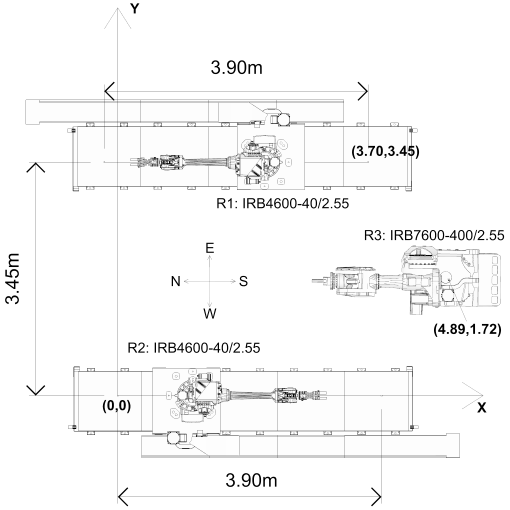
\includegraphics [trim={0cm 0cm 0cm 0cm}, clip, width=0.90\linewidth]{fig1_fabcell}
            \caption{Layout of the three-robot cooperative fabrication cell with North defined towards the left.}
    	\label{fig:fig1_fabcell} 
    \end{figure}

     The computational workflow relies on the COMPAS framework \citep{mele_compas_2017}. Robotic fabrication processes are planned and executed using the COMPAS FAB package in conjunction with a ROS backend \citep{rust_compas_2018}. The execution of robotic motion commands is facilitated through COMPAS RRC \citep{fleischmann_compas_2020}, and the corresponding RRC driver operates on the IRC5 controller.
    
\subsection{Experimental Prototype} \label{sec:3a_prototype}
    At the heart of this research project is a prefabricated physical prototype - a timber shed structure constructed in accordance with conventional American stick frame construction practices. This prototype serves as a representative example of an existing structure that will undergo robotic disassembly and reassembly, demonstrating the real-world application of the computational methods developed in this research. Illustrated in \Cref{fig:fig2_shed_structure}, the structure has dimensions of 8 x 6 ft ($\sim$2.4 x 1.8 m) in plan, a stud wall height of 8.0 ft ($\sim$2.6 m), and a crown height of 9.6 ft ($\sim$2.9 m). Constructed using 2x4" and 2x6" SPF dimensional lumber, the traditional planar wall sheathing is replaced with linear members positioned diagonally across the stud wall to impart the necessary shear stiffness.

    \begin{figure}[ht]
    	\centering
    	\begin{subfigure}[b]{0.49\linewidth}
    		\centering
    		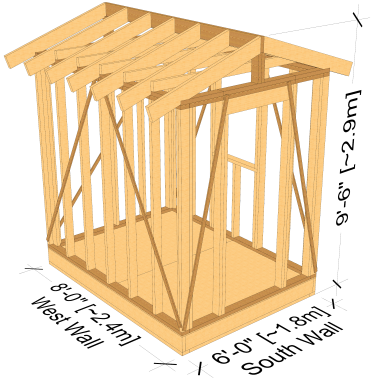
\includegraphics [trim={0cm 0cm 0cm 0cm}, clip, width=0.99\textwidth]{fig2_shed}
            \caption{Rendering of the structure showing the dimensions and naming convention for the walls.}
    	\end{subfigure}
        %
    	\begin{subfigure}[b]{0.49\linewidth}
    		\centering
    		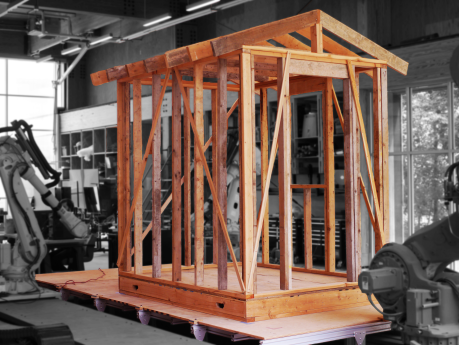
\includegraphics [trim={0cm 0cm 0cm 0cm}, clip, width=0.99\textwidth]{fig2_shed_photo}
            \caption{Image of structure showing its placement in the robotic work cell (from \cite{bruun_zerowaste_2022}).}
    	\end{subfigure}
        %
    	\caption{The prototype timber structure.}
    	\label{fig:fig2_shed_structure} 
    \end{figure}

    To streamline the forthcoming presentation of results and discussion regarding robotic fabrication sequences, the overall prototype structure is represented as a composite of distinct sub-structures - namely, the four walls (East, West, North, South) and the roof. Each of these sub-structures is then comprised of individual linear members, systematically labeled, and color-coded according to their respective types as shown in \Cref{table:shed_members}. The color-coded members and the five sub-structures are depicted in \Cref{fig:fig3_shed_members}, where the individual members are labelled using the following convention $AB\#\_\$$, where:

    \begin{itemize}
        \item [A:] The first letter indicates if it is part of the roof (R) or one of the four walls (N, S, E, W).
        \item [B:] The second letter represents the type of member, as shown in the 2nd column of \Cref{table:shed_members}.
        \item [\#:] The third digit is used to number a unique member of a particular type.
        \item [\$:] The fourth digit (if required) is used to number a section of a single member.
    \end{itemize}

    The color-coding and member notation described in \Cref{table:shed_members} and \Cref{fig:fig3_shed_members} matches the topological support hierarchy representation, which is introduced in \Cref{sec:4b_topo}. This convention is consistently used in all the subsequent results and discussions in the chapter.

    \begin{figure}[H]
    	\centering
    		\centering
    		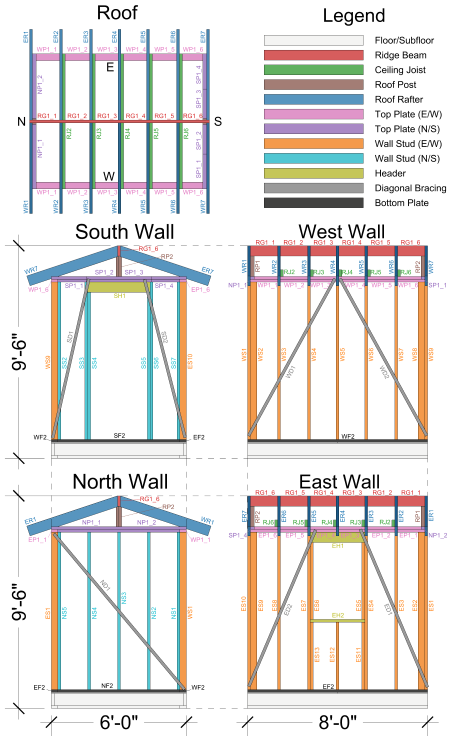
\includegraphics [trim={0cm 0cm 0cm 0cm}, clip, width=0.70\linewidth]{fig3_shed_members}
            \caption{Prototype structure shown as an assembly of five sub-structures with the members in each color-coded according to their type.}
    	\label{fig:fig3_shed_members} 
    \end{figure}


\begin{table}[ht]
    	\renewcommand{\arraystretch}{1.4}
    	\footnotesize
    	\centering
    	\caption{Members in the prototype structure}
    	% \vspace{-2.5mm}
    	
    	\begin{tabular}{m{0.01cm}m{2.5cm}m{1.0cm}m{1.0cm}m{1.0cm}}
    		\specialrule{.10em}{0.2em}{.2em}
    		\centering
    		%
    		\phantom{}%to space out the top headings nice
    		&\multicolumn{1}{l}{\bf{Member}}
    		&\multicolumn{1}{c}{\bf{Letter}}
            &\multicolumn{1}{c}{\bf{Count}}
    		&\multicolumn{1}{l}{\bf{Color}}
    		\\	
    		%
    		\specialrule{0.06em}{0.2em}{.2em}
    		%
            &\makecell[lc]{Floor}%
            &\makecell[cc]{N/A}%
            &\makecell[cc]{N/A}%
    		&\makecell[lc]{white}%
            \\ \cmidrule{1-5}
            %
    		&\makecell[lc]{Roof Girder}%
            &\makecell[cc]{G}%
    		&\makecell[cc]{1}%
    		&\makecell[lc]{red}%
            \\ \cmidrule{1-5}
            %
        	&\makecell[lc]{Ceiling Joist}%
            &\makecell[cc]{J}%
    		&\makecell[cc]{5}%
    		&\makecell[lc]{green}%
            \\ \cmidrule{1-5}
            %
    		&\makecell[lc]{Roof Post}%
            &\makecell[cc]{P}%
    		&\makecell[cc]{2}%
    		&\makecell[lc]{brown}%
            \\ \cmidrule{1-5}
            %
    		&\makecell[lc]{Roof Rafter}%
            &\makecell[cc]{R}%
    		&\makecell[cc]{14}%
    		&\makecell[lc]{blue}%
            \\ \cmidrule{1-5}
            %
            &\makecell[lc]{Top Plate (E/W)}%
            &\makecell[cc]{P}%
    		&\makecell[cc]{2}%
    		&\makecell[lc]{pink}%
            \\ \cmidrule{1-5}
            %
            &\makecell[lc]{Top Plate (N/S)}%
            &\makecell[cc]{P}%
    		&\makecell[cc]{2}%
    		&\makecell[lc]{purple}%
            \\ \cmidrule{1-5}
            %
            &\makecell[lc]{Wall Stud (E/W)}%
            &\makecell[cc]{S}%
    		&\makecell[cc]{22}%
    		&\makecell[lc]{orange}%
            \\ \cmidrule{1-5}
            %
            &\makecell[lc]{Wall Stud (N/S)}%
            &\makecell[cc]{S}%
    		&\makecell[cc]{12}%
    		&\makecell[lc]{cyan}%
            \\ \cmidrule{1-5}
            %
            &\makecell[lc]{Header}%
            &\makecell[cc]{H}%
    		&\makecell[cc]{3}%
    		&\makecell[lc]{yellow}%
            \\ \cmidrule{1-5}
            %
            &\makecell[lc]{Diagonal Bracing}%
            &\makecell[cc]{D}%
    		&\makecell[cc]{7}%
    		&\makecell[lc]{grey}%
            \\ \cmidrule{1-5}
            %
            &\makecell[lc]{Bottom Plate}%
            &\makecell[cc]{F}%
    		&\makecell[cc]{4}%
    		&\makecell[lc]{black}%
            \\
            %
    		\specialrule{0.10em}{0.2em}{.2em}
    		%
    	\end{tabular}
    	\label{table:shed_members}
    \end{table}



\subsection{Project Phases} \label{sec:3b_phases}
    The ZeroWaste project aims to develop an integrated computational workflow for orchestrating a cooperative, scaffold-free robotic disassembly and reassembly process on an unknown existing structure. The practical manifestation of this goal involves a series of physical demonstrations on the prototype timber structure described in \Cref{sec:3a_prototype}. The overall project is strategically divided into three distinct fabrication phases, each serving as a milestone to incrementally evaluate the developed methods described in \Cref{sec:4_experimental_methods}. Each phase demonstrates increasing complexity in both the structural disassembly and reassembly tasks and the degree of cooperative robotic sequencing necessary to execute these tasks. These phases are as follows: Phase 1, single target member removal; Phase 2, full wall disassembly and partial reassembly; Phase 3, full wall removal and reassembly. Further details and the results of these fabrication phases are presented in \Cref{sec:5_results}.



% ----------------------------------------------------------------------------------------------------
% 4. Experimental Methods
% ----------------------------------------------------------------------------------------------------
\section{Workflow and Methods} \label{sec:4_experimental_methods}
    The overarching computational workflow utilized across all phases of the ZeroWaste project is illustrated in \Cref{fig:fig4_workflow}, depicting three primary components. Firstly, the use of 3D cameras mounted on robots to capture geometric and positional data pertaining to the unknown existing timber structure, which is here represented by the prototype shed (\cref{sec:4a_camera}). Secondly, calculation of potential cooperative robotic disassembly and reassembly sequences when given user-specified member targets. This is achieved by leveraging the topological member support hierarchy representation of the structure (\cref{sec:4b_topo}). Lastly, the workflow incorporates an evaluative process, assessing the feasibility of generated fabrication sequences, given the generated geometric data on the structure, regarding both structural performance and constraints associated with robotic reach and path planning (\cref{sec:4c_feasible}).

    \begin{figure}[ht]
    	\centering
    		\centering
    		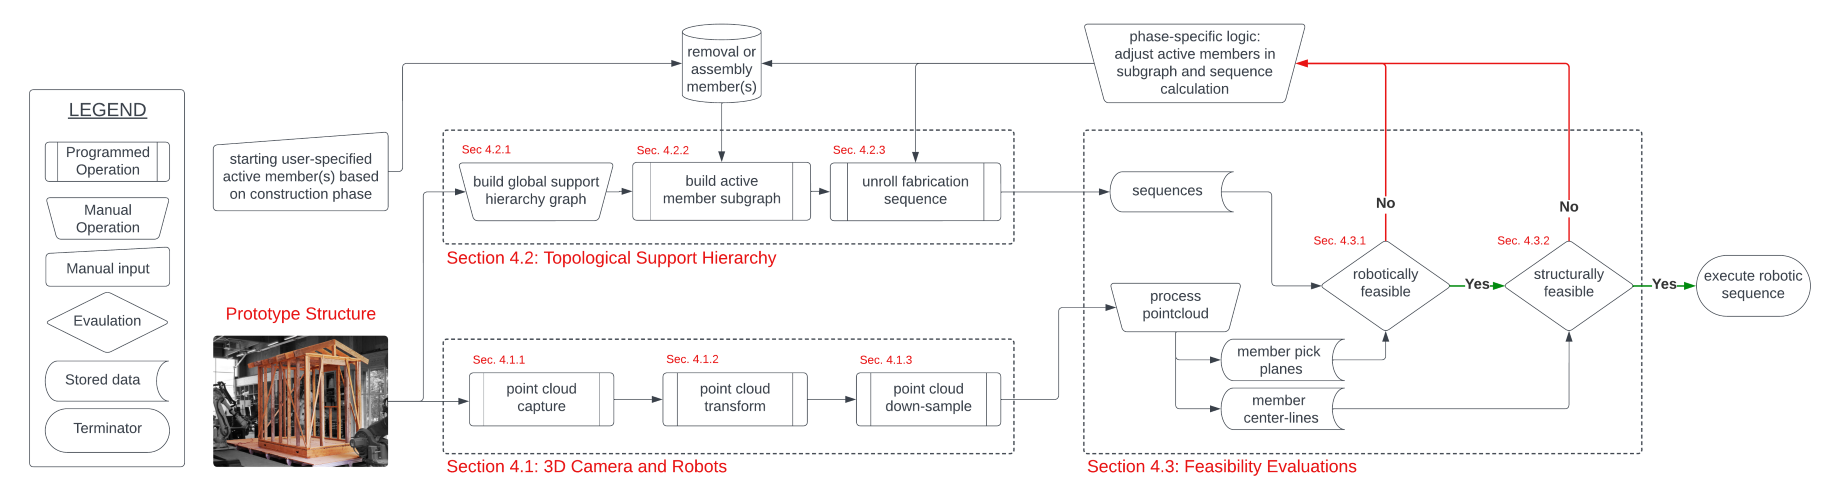
\includegraphics [trim={0cm 0cm 0cm 0cm}, clip, width=0.99\linewidth]{fig4_workflow}
            \caption{Computational workflow showing the interaction between the methods described in \Cref{sec:4_experimental_methods}.}
    	\label{fig:fig4_workflow} 
    \end{figure}

\subsection{3D Camera and Robots} \label{sec:4a_camera}
    Each of the two IRB4600 robots, positioned on tracks, is equipped with a Zivid 3D structured light camera with a spatial resolution of 0.39 mm at a distance of 700 mm \citep{zivid_as_zivid_2021}. The initial phase of the project involved creating a point cloud of the entire existing structure, which is a composite stitched together from several independent camera captures taken at various locations around the structure. Performing this procedure is essential before initiating any fabrication processes since an accurate digital representation of the as-built geometry of the unknown structure is required. Even if a pre-existing digital model of the structure is available, as is the case with the prototype structure, this point cloud step must still be performed as the as-built conditions of the structure invariably differ from the perfect digital model.

    Moreover, beyond generating an accurate geometric representation of the structure, accurately positioning this geometry within the workcell is equally vital. This requires that the structure is correctly situated with respect to robots. Precise relative positioning is essential for the execution of robot move commands, which are sent relative to robots' base coordinate frame - that is, where the robot perceives its spatial location to be. Therefore, maintaining alignment between the as-built digital representation of the real structure and the perceived location of the robots in the fabrication cell is crucial for the execution of all robotic movements. 

    \subsubsection{Point Cloud Capture} 
        To construct an accurate as-built model of the structure, the robots capture 3D images from different spatial positions as they move around the structure (R1 = 105, R2 = 62 separate positions). Each capture generates a unique point cloud. The individual point clouds are then transformed to the correct global coordinate frame and combined into a single point cloud representing the whole structure, shown in \Cref{fig:fig5_pointcloud}.

        \begin{figure}[ht]
        	\centering
        		\centering
        		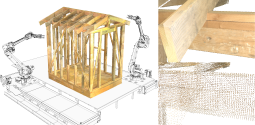
\includegraphics [trim={0cm 0cm 0cm 0cm}, clip, width=0.99\linewidth]{fig5_pointcloud}
                \caption{As-built point cloud of the prototype structure from combined individual captures transformed to the correct location in space with respect to the robotic cell (left). Point cloud density for a small region of the structure before (top-right) and after (bottom-right) down-sampling with low-definition settings.}
        	\label{fig:fig5_pointcloud} 
        \end{figure} 

    \subsubsection{Point Cloud Transform} 
       The cameras are mounted on the robots used for the fabrication tasks, which is known as an eye-in-hand setup. Since the Tool Center Point (TCP) location with respect to the robot base is always known by the robot controller, this can be used to perform coordinate transforms on point clouds captured by the fixed camera. A point in the camera's coordinate system (i.e., how the camera sees the object), $P_{object\_camera}$, can be transformed to a point in the global coordinate frame of the CAD model, $P_{object\_world0}$, aligned with where the robots are situated in the global coordinate frame in the following manner:
    
         \begin{equation*}
             P_{object\_world0} = H_3 * H_2 * H_1 * P_{object\_camera}
         \end{equation*}
    
        Where the 4x4 transformation matrices are the following:
    
        \begin{itemize}
            \item [H1:] from TCP to camera. This transformation is calculated from a single eye-in-hand calibration routine that must be performed only once each time the camera is re-mounted.
            \item [H2:] from robot base to TCP. This transformation is calculated from the positional frame representing the TCP, which is queried from the robot controller using the COMPAS RRC API \citep{fleischmann_compas_2020} at each camera capture.
            \item [H3:] from World0 to Work Object (WOBJ) frame. This transformation is calculated from an user-defined coordinate frame set for each robot. This frame serves to establish a unified coordinate system for all the robots in multi-robot process, aligning them with the global coordinate frame of the CAD model. Consequently, all positional data is defined relative to this unified coordinate system.
        \end{itemize}

    \subsubsection{Point Cloud Down-Sample} 
        The 3D cameras have a resolution that results in captured point clouds with greater fidelity than is strictly necessary for the subsequent robotic processes. Individual captures range from 50-200k points, resulting in raw combined point cloud model with 23.6M points (R1 = 14.5M and R2 = 9.1M points). A model of this size is computationally expensive to work with. In addition, the process of combining separate captures also leads to overlapping regions with duplicated points. Thus, further processing to reduce the overall point cloud density and remove the unnecessary duplicate points is required.

        The raw point cloud undergoes down-sampling using statistical outlier, radius outlier, and voxel filters from the open3D package library \citep{zhou_open3d_2018}. The hyper-parameters for this process are shown in \Cref{table:pcd_downsample}, where the more aggressive low-definition (LD) settings result in a coarse overall model with only 0.55 million points, while the high-definition (HD) settings result in a model with 11.8M points. A final manual clean to remove unnecessary points, such as the ground, or any visible missed outliers, further reduces the model size slightly. The smaller LD model is used in computational processes where working with a minimal dataset is crucial, while the higher quality HD model is suitable for visual applications.

        \begin{table}[ht]
        	\renewcommand{\arraystretch}{1.5}
        	\normalsize
        	\centering
        	\caption{Hyper-parameters and results for low-definition (LD) and high-definition (HD) down-sampling procedures}
        	
        	\begin{tabular}{l |c cc}
        		\specialrule{.10em}{0.2em}{.2em}
        		\centering
        		%
        		\phantom{a}
        		&\phantom{\makecell{\vspace{0.5em}}}%to space out the top headings nice
                &\multicolumn{1}{c}{LD}
                &\multicolumn{1}{c}{HD}
        		\\	
        		\specialrule{0.06em}{0.2em}{.2em}
        		%
                pcd (start) && 23.6M &23.6M\\
        
                \specialrule{0.06em}{0.2em}{.2em}
                
        		voxel\_size (m) & &0.010 &0.001\\
                nb\_neighbor & &30 &20 \\
                std\_ratio & &1.0 &2.0 \\
                nb\_points & &20 &20 \\
                radius (m) & &0.08 &0.08 \\
        
                \specialrule{0.06em}{0.2em}{.2em}
                
                pcd (down-sample) &&0.6M &11.8M \\
                pcd (manual clean) &&0.5M &11.3M \\
        		\specialrule{0.10em}{0.2em}{.2em}
        		%
        	\end{tabular}
        	
        	\label{table:pcd_downsample}
        \end{table} 

        
        \Cref{fig:fig5_pointcloud} displays the final stitched model of the as-built prototype structure accurately located with respect to the robotic cell after the process of transformation and down-sampling. This image also illustrates the difference in the density between the raw and down-sampled point clouds for a small region of the structure.



\subsection{Topological Support Hierarchy} \label{sec:4b_topo}
    Creating a computational framework to plan disassembly and reassembly sequences that are both stable and feasible requires a robust representation of the interconnections and support relationships within a structure. One effective method for visualizing this connectivity is using a multidirected graph (multidigraph) data structure \cite{valiente_algorithms_2021}. In the context of this research, a representation referred to as the topological support hierarchy graph was developed. In this graph, individual members are depicted as vertices, while physical connections between members are represented as edges. The direction of support is indicated by outgoing edges, effectively portraying the load-path.
    
    However, representing geometric information, such as where along a member (e.g., a top plate) multiple members are being supported, poses a challenge in a topological data structure like a graph. To address this challenge, a more detailed and precise graph representation by decomposing certain elements into their constituent submembers is proposed. Each submember is then treated as an independent vertex in the graph. To signify their mutually supportive relationship, vertices corresponding to submembers of the same member are connected by two parallel, opposing edges -— a situation referred to as a fixed connection.

    \Cref{fig:fig6_topo} illustrates the methodology for how a structure can be represented as a topological support hierarchy graph, for two members (B) supported by members (A and C). This graph representation can be further refined by dividing members A and C into submembers, providing a more nuanced depiction of how individual members are supported within the structure.

    \begin{figure}[ht]
        \centering
            \centering
            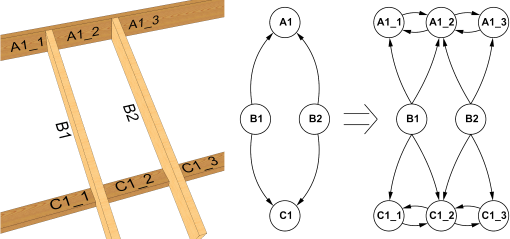
\includegraphics [trim={0cm 0cm 0cm 0cm}, clip, width=0.99\linewidth]{fig6_topo}
            \caption{Directed edges show that members B1, B2 are supported by members A1 and C1. These support members can also be shown subdivided into their constituent submembers that are connected with parallel and opposite edges to represent a fixed connection.}
        \label{fig:fig6_topo} 
    \end{figure} 

    \subsubsection{Build Global Support Hierarchy Graph}
        \begin{figure}[ht]
        	\centering
        		\centering
        		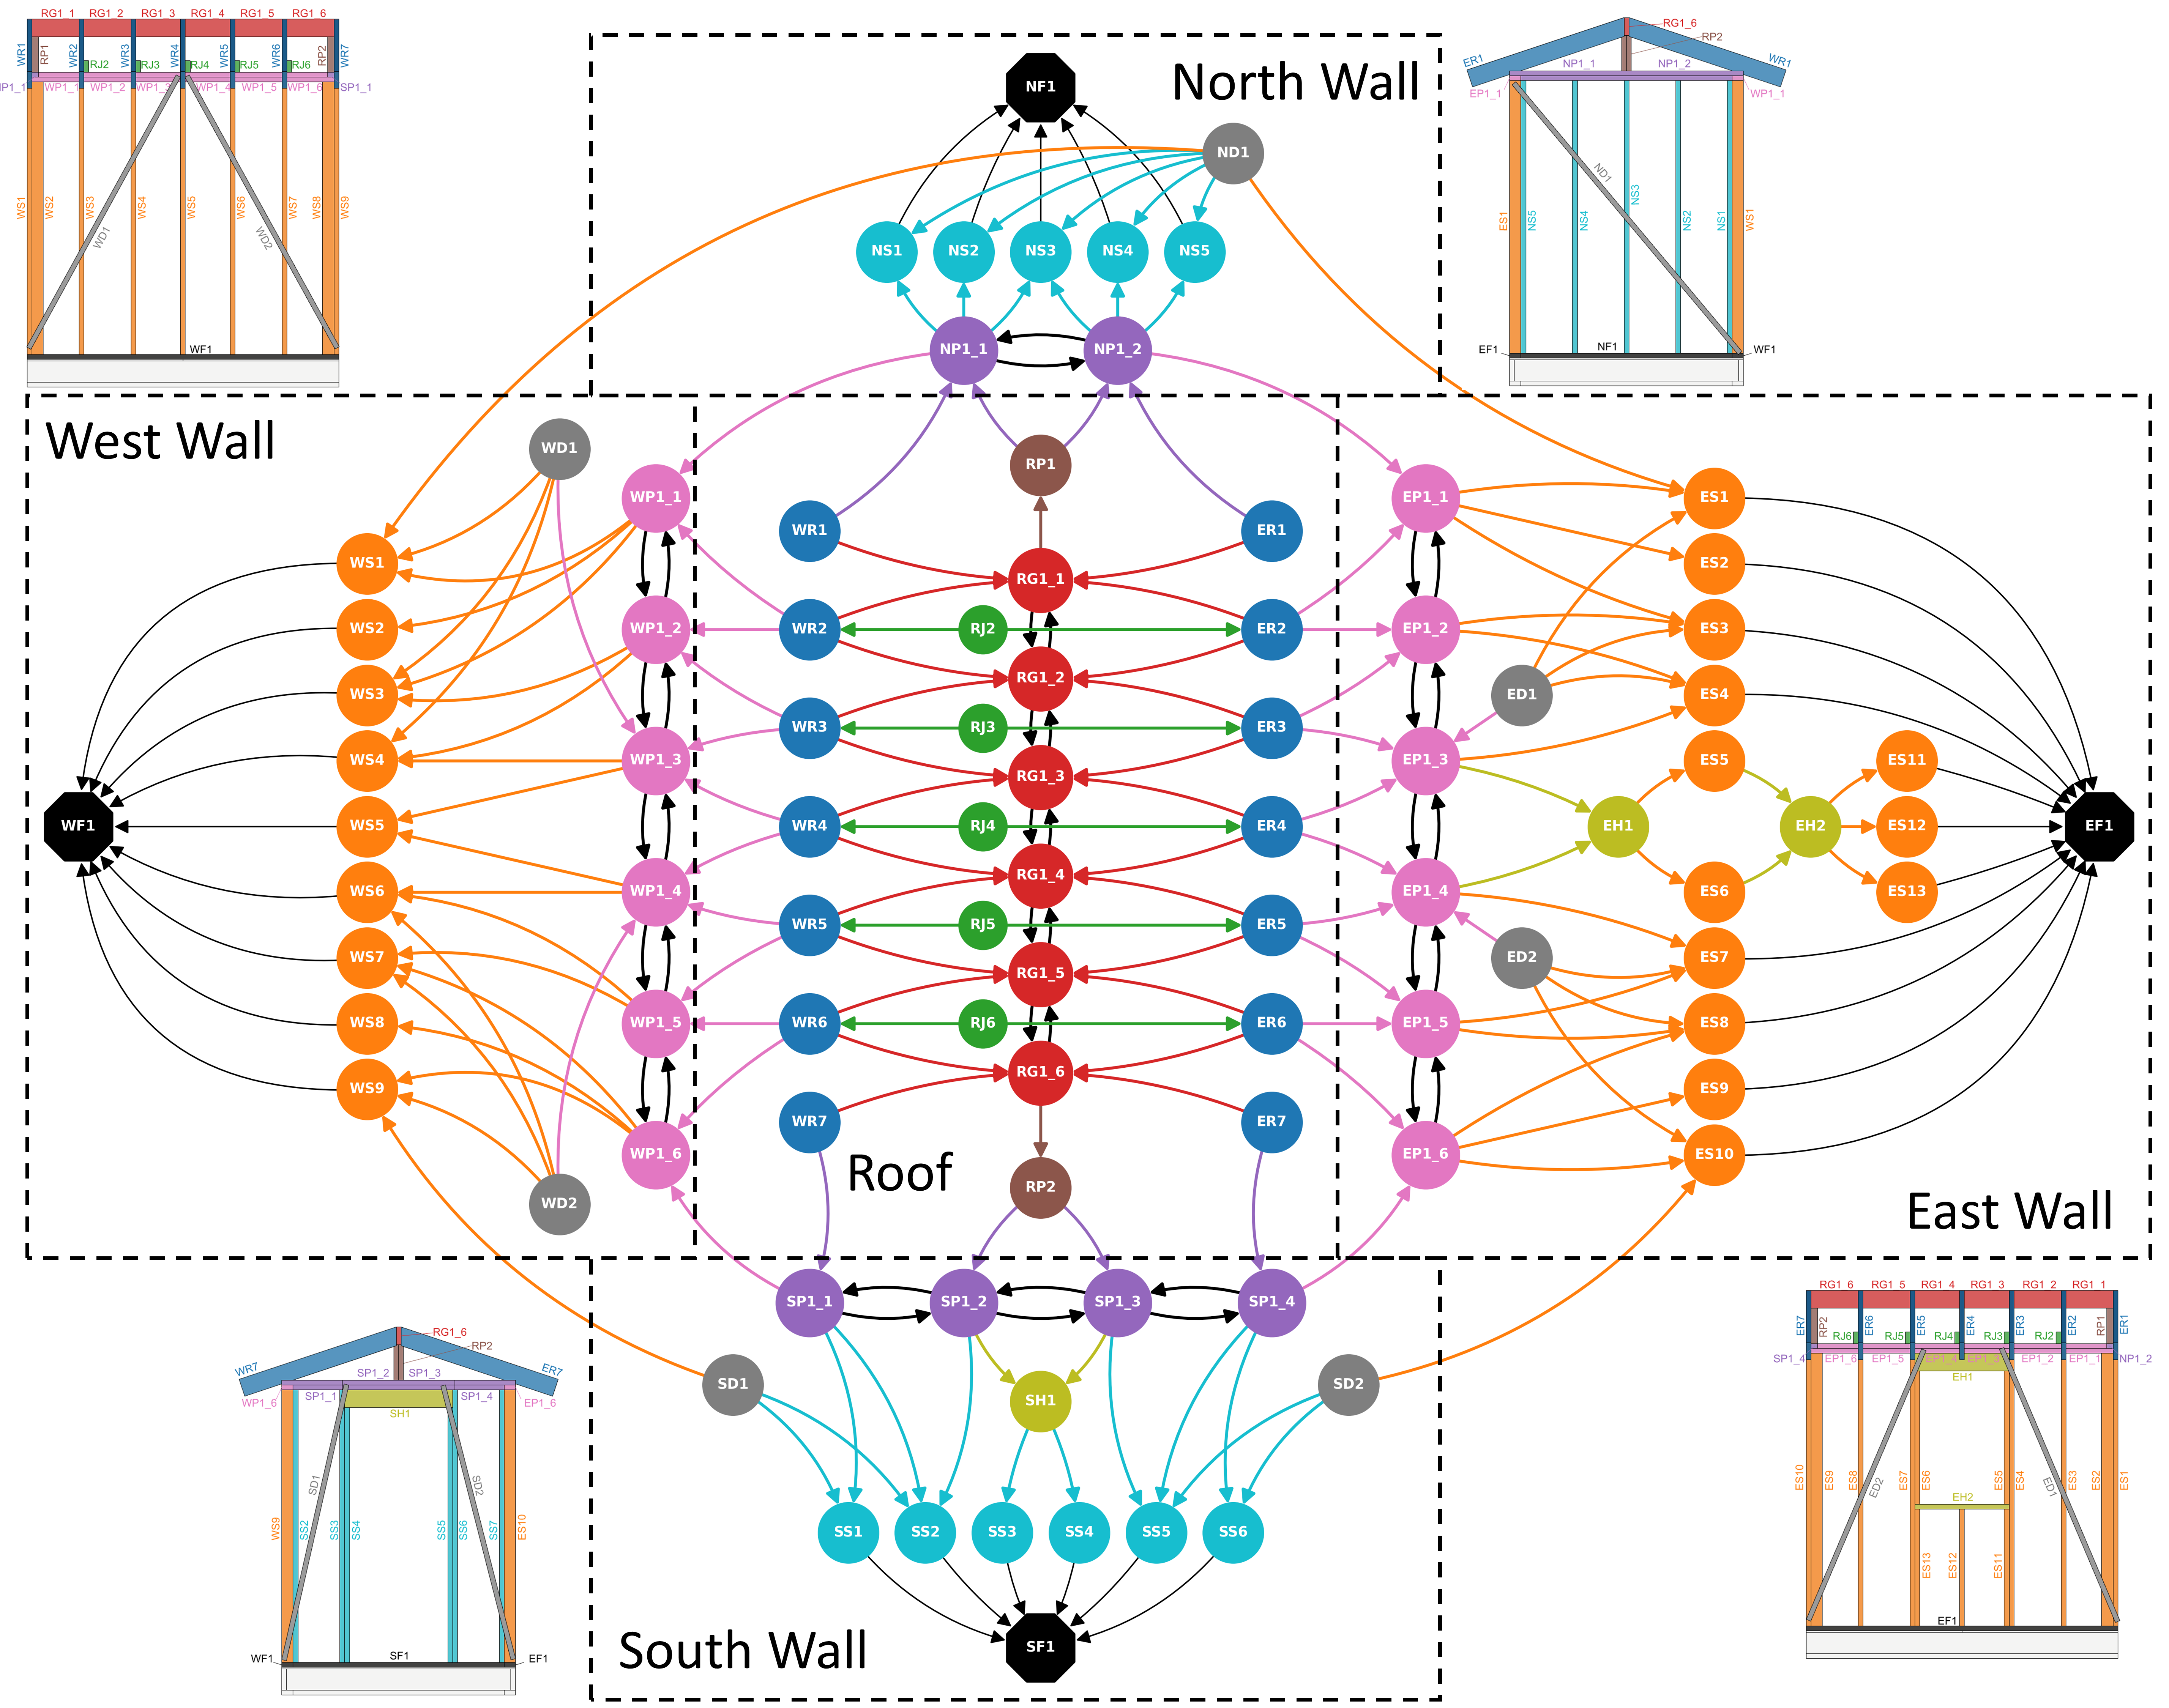
\includegraphics [trim={0cm 0cm 0cm 0cm}, clip, width=0.99\linewidth]{fig7_full_graph}
                \caption{The global connection hierarchy in the timber prototype structure is represented as a multidirected graph with outgoing edges indicating the direction of support. The graph is organized into five regions, where the names and colors of the vertices are based on the convention introduced in \Cref{sec:3a_prototype}.}
        	\label{fig:fig7_full_graph} 
        \end{figure} 

        The global support hierarchy graph representing the entire prototype structure, which is an input to the computational processes for planning robotic fabrication sequences, is shown in \Cref{fig:fig7_full_graph}. Constructed manually, this graph adheres to the principles illustrated in \Cref{fig:fig6_topo}. Vertex names and colors are aligned with the member naming and color scheme described in \Cref{sec:3a_prototype}, while edges are color-coded based on their originating vertices. To more accurately capture the support hierarchy of the numerous individual members supported on them, the top plate and roof ridge beam members are represented as a series of submembers with fixed supports between them.
        
        The graph in \Cref{fig:fig7_full_graph} visually partitions the structure into five distinct regions, either the roof or one of the four walls. However, this segmentation is primarily for clarity since the relative positioning of vertices lacks significance, as a graph data structure exclusively conveys topological information. The structure terminates at the foundation supports, visually shown in the graph by hexagonal vertices that represent the connection between the bottom plate of each wall and the ground beneath.
            
    \subsubsection{Build Active Member Subgraphs} \label{sec:4b_topo_2}
        Given an active member, such as a target specified for removal, an algorithmic operation can be executed on the global support member hierarchy graph of the entire structure. This procedure yields a subgraph encompassing the members that are directly affected during the removal of the active member. 

        This procedure is based on a customized breadth-first search algorithm \citep{valiente_algorithms_2021}, which is used to traverse the regions in the global support hierarchy graph adjacent to the vertex representing the target member. The rationale for this search approach is that achieving a feasible disassembly sequence without leaving unstable or disconnected components in the structure is higher when all members in the region connected to the target member are also removed or identified as requiring some form of temporary support to during the overall removal process. For instance, if an active member is supporting several other members, it is logical to remove these supported members first as it is unlikely that they will remain structurally stable upon the removal of the active member. Thus, a breadth-first search is used to identify whether a member actively supports or is supported by other members, a condition represented by incoming and outgoing edges from neighboring vertices. Thus, any members connected to the active member will become part of the overall disassembly sequence. This procedure is then iterated to identify the members in turn supported by these intermediate members, resulting in a subgraph of the global support hierarchy graph that represents all the affected members in for a user-specified active member.

        The process of calculating subgraphs for individual user-specified active members is shown in \Cref{alg:alg1_single}, with the breadth-first search performed in the \textit{calc\_subg} function (\cref{sec:appendixa_1}). When multiple user-specified active members are indicated for a single disassembly procedure, there is no need to repeat the breadth-first search. Instead, as shown in \Cref{alg:alg2_multi}, the subgraphs representing the individual members can be joined to produce the subgraph for the multiple active member case. All graph-based computational processes are performed using the NetworkX package for Python \citep{hagberg_exploring_2008}.


        \begin{algorithm}
            \setstretch{1.05}
            \caption{Single Member Subgraph(s) Calc}
            \label{alg:alg1_single}
            \begin{algorithmic}[1]
            \Procedure{bld\_subg\_single}{G, rms}
                \State Ks $\gets$ []
                \State
                \For{rm \textbf{in} rms}
                    \State K $\gets$ \textit{calc\_subg}(G.copy(), rm)
                    \State n\_cut $\gets$ \textit{fxd\_nodes\_cut}(G, K)
                    \State \textit{fxd\_nodes\_support}(G, K, rm, n\_cut)
                    \State Ks.append(K)
                \EndFor
                \State
                \State \textbf{return} Ks
            \EndProcedure
            \end{algorithmic}
        \end{algorithm}

        \begin{algorithm}
            \setstretch{1.05}
            \caption{Multi-Member Subgraph Calc}
            \label{alg:alg2_multi}
            \begin{algorithmic}[1]
            \Procedure{bld\_subg\_multi}{G, Ks, rms}
                \State K\_joined $\gets$ nx.compose\_all(Ks)
                \State \textit{add\_in\_extra\_edge}(G, K\_joined)
                \State n\_cut $\gets$ \textit{fxd\_nodes\_cut}(G, K\_joined)
                \State \textit{fxd\_nodes\_support}(G, K\_joined, rms, n\_cut)
                \State \textbf{return} K\_joined
            \EndProcedure
            \end{algorithmic}
        \end{algorithm}

        The breadth-first search concludes when the vertex-checking queue is empty. This occurs before traversing the entire graph due to certain conditions that lead to a vertex being labelled as an end, meaning its neighbors are not examined. For instance, a vertex with only outgoing edges implies that the member it represents can be removed without impacting any other parts of the structure. Conversely, a vertex with only incoming edges designates a foundation support vertex that will not be removed.
        
        The end condition is also triggered for any vertex possessing at least one fixed edge (i.e., equal and opposite parallel edges), indicating that it represents a submember. However, additional logic is necessary to determine whether these submembers qualify as valid end supports. A submember with only one fixed connection, designating it as the terminal segment of a larger member, may pose a potential stability hazard and requires further scrutiny. If such a submember shares a sole unidirectional edge with an active member, it necessitates removal, thus being treated as a standard vertex to be added to the breadth-first search queue. Alternatively, the submember may also require removal if all its edges are found in the subgraph, a condition verified in the $fxd\_nodes\_cut$ function (\cref{sec:appendixa_2}). Otherwise, the submember is considered adequately supported and remains in the structure acting as an end support in the subgraph.

        In the $fxd\_nodes\_support$ function, all the ends that remain in the structure (i.e., submembers with fixed connections) are checked for adequate support at the culmination of the removal process (\cref{sec:appendixa_2}). Adequate support is defined by the requirement that at least two supports (i.e., outgoing edges) persist in the global support hierarchy graph once the subgraph has been deleted. For example, a submember with two fixed connections, signifying its placement within the interior of a larger member, is considered adequately supported. This condition serves as a safeguard against the formation of structurally undesirable cantilevered segments within the remaining structure after the disassembly process is completed. This is checked in both the single and multi-member subgraph procedures outlined in \Cref{alg:alg1_single,alg:alg2_multi}.

        \Cref{fig:fig8_example_subgraphs} shows example subgraphs calculated using the computational procedures outlined in this section given different user-specified targets: east side rafter \#2 (ER2), east side stud \#10 (ES10), north side top plate submember \#1 (NP1\_1), east side top plate submember \#2 (EP1\_2), and the composite of west side stud \#3 (WS3) + west top plate submember \#2 (WP1\_2). The colors for the edges and vertices in these subgraphs no longer indicate the physical member type, but instead represent output related to how the edges and vertices have been labelled in the computational process when generating the subgraph. For example, black is used for end members and green is used for start members. The shape of the vertices is also used to distinguish between different conditions. If an edge is black it represents typical support between members, but dashed red edges indicate that a submember will require physical cutting from the overall member it is a part since it must be removed in the disassembly process. The complete legend for the nodes and edges are labelled in the active member subgraphs is shown in \Cref{fig:fig8_example_subgraphs}. 

        \begin{figure}[ht]
        	\centering
        		\centering
        		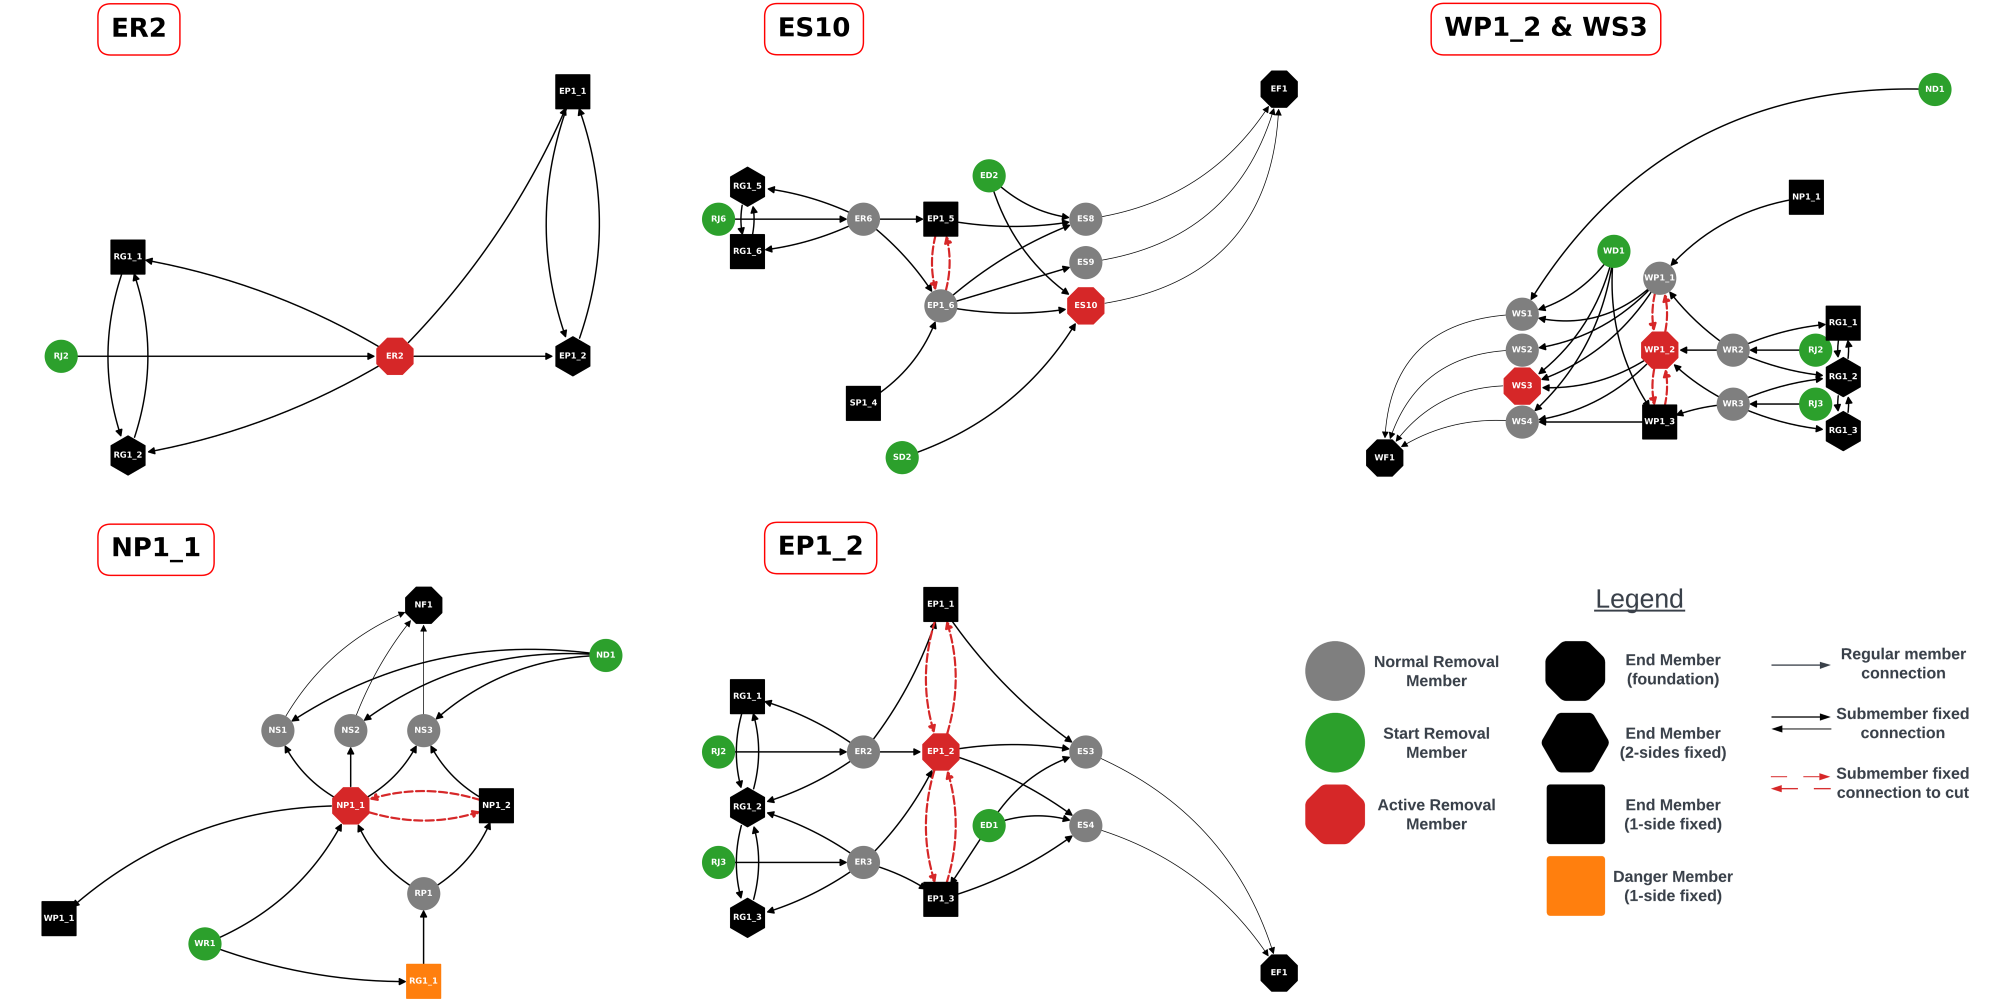
\includegraphics [trim={0cm 0cm 0cm 0cm}, clip, width=0.99\linewidth]{fig8_subgraphs_example}
                \caption{Examples of active member subgraphs constructed using the algorithmic procedures described in \Cref{sec:4b_topo_2}. Vertices and edges are drawn to represent the different conditions as per the legend.}
        	\label{fig:fig8_example_subgraphs} 
        \end{figure} 

    \subsubsection{Calculate Fabrication Sequences}
        A computational procedure is employed to calculate a set of potential fabrication sequences, utilizing an active member subgraph generated through the methodology outlined in \Cref{sec:4b_topo_2}. Conceptually, this involves unfolding the subgraph data structure into a linear sequence of discrete fabrication steps. The overarching method for generating these sequences is summarized in \Cref{alg:alg3_sequence}, with supplementary functions further explained in \Cref{sec:appendixa_3}.

        \begin{algorithm}
            \setstretch{1.05}
            \caption{Unroll subgraph into sequence}
            \label{alg:alg3_sequence}
            \begin{algorithmic}[1]
            \Procedure{bld\_sequence}{K, rms, num\_agents}
                \State saved\_K, saved\_seq $\gets$ [],[]
                \State n\_active\_type $\gets$ [``start'',``rob\_sprt'']
                \State
                \While{True}
                    \State n1 $\gets$ \textit{find\_n\_active}(K, n\_active\_type)
                    \State n2 $\gets$ \textit{set\_new\_to\_rob\_support}(K)
                    
                    \State
                    \If {n1 $\cup$ n2 \textbf{is} $\emptyset$}
                        \State terminate loop
                    \EndIf
                    
                    \State
                    \State n\_rmv,n\_rob\_sprt $\gets$ \textit{select\_n\_active}(n1,n2)

                    \State
                    \State saved\_K.append(K)
                    \State saved\_seq.append(n\_rmv)
                    
                    \State 
                    \State K.remove\_nodes\_from(n\_rmv)
                    \State K $\gets$ \textit{new\_subg\_relabel}(K, rms)

                \EndWhile
            \State \textbf{return} saved\_K, saved\_seq
            \EndProcedure
            \end{algorithmic}
        \end{algorithm}

        The algorithm locates start vertices in the subgraph describing the full fabrication sequence. These vertices are first saved as a discrete disassembly step and then removed from the subgraph to represent the physical process occurring. The remaining subgraph is then relabeled with new start nodes to account for the resulting changes in the support hierarchy after this step is executed. This process of locating, removing, relabeling is iterated on the subgraph until all nodes are removed. The objective is to optimize the removal of the maximum number of members in a single step, corresponding to the available robotic agents. In cases where the number of start nodes exceeds the count of robotic agents at a given step, a sequence is generated for each permutation. Subsequently, this exhaustive set of sequences is evaluated as outlined in \Cref{sec:4c_feasible}, to ascertain feasibility in terms of structural behavior and robotic reachability.

        \Cref{fig:fig9_example_sequence} illustrates a representative outcome of the fabrication sequence calculation process applied to the WP1\_2 \& WS3 active member subgraph, as shown depicted in \Cref{fig:fig8_example_subgraphs}. These calculations consider the presence of two robotic agents, thus allowing the removal of a maximum of two members per step. In step \#1, more than two start vertices are identified, implying the existence of multiple permutations at this stage, where the displayed sequence represents just one of these possibilities. All end nodes (depicted in black) are retained in the sequence graphs for better visualization; these nodes are not isolated components but are interconnected and adequately supported by the remaining structure beyond the boundaries of the specific subgraph.

        \begin{figure}[ht]
        	\centering
        		\centering
        		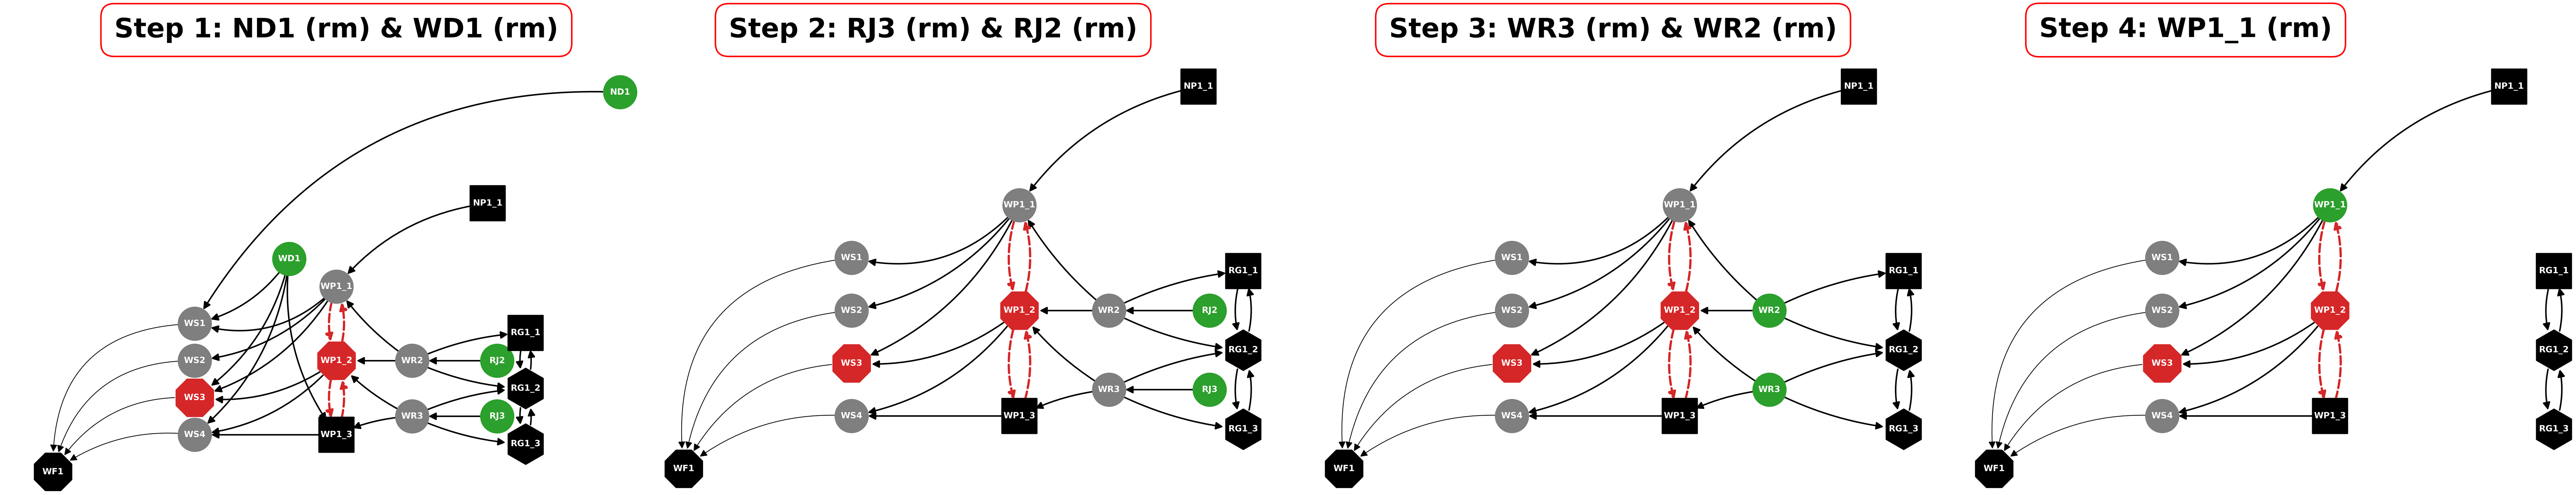
\includegraphics [trim={0cm 0cm 0cm 0cm}, clip, width=0.99\linewidth]{fig9_sequence_example}
                \caption{Example of a partial disassembly sequence (four steps) calculated from the subgraph for active members WP1\_2 \& WS3. After each step the subgraph is relabeled with new start nodes in green.}
        	\label{fig:fig9_example_sequence} 
        \end{figure} 


    
\subsection{Feasibility Evaluations} \label{sec:4c_feasible}
    The computational methods discussed in the preceding \Cref{sec:4b_topo}, rooted in the topological support hierarchy representation of the structure, generate a sequence of fabrication plans when provided with a set of active members. The primary goal at this stage is just to discern fabrication sequences that could potentially be executed without external scaffolding while ensuring structural stability. Subsequently, these candidate sequences must undergo further examination, considering the physical structure itself, to verify feasibility and identify the optimal sequence.
    
    An analysis of the generated sequences, evaluating both structural and robotic feasibility, precedes the selection of a sequence for execution. The verification process involves two concurrent procedures applied to the accurate as-built point cloud gathered as per the methods described in \Cref{sec:4a_camera}. Firstly, the validation of robotic path planning and reachability is conducted using the COMPAS and COMPAS FAB package with a ROS backend \citep{rust_compas_2018,mele_compas_2017}. Secondly, a detailed parametric finite element (FE) analysis of the structure is carried out in Rhino/Grasshopper with Karamba3D \citep{rutten_grasshopper_2007, preisinger_karambatoolkit_2014} to assess the structural behavior at each step in the fabrication sequence.
    
    \subsubsection{Robotic Feasibility}
        \begin{figure}[ht]
            \centering
            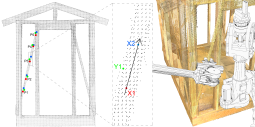
\includegraphics [trim={0cm 0cm 0cm 0cm}, clip, width=0.99\linewidth]{fig10_pick_locations}
            \caption{Left: Five pick locations (P1 - P5) on a member are manually initialized from the as-built point cloud of the structure. Middle: At each location three points are used to define a spatial plane for the robot to reach. Right: Inverse kinematic path planning checks reveal that only P3 is reachable by a robot without encountering collisions with the structure or other robots in the work cell.}
        	\label{fig:fig10_pick_locations} 
        \end{figure} 
        
        The first procedure involves assessing the physical executability of a proposed sequence from the robotic perspective. This evaluation focuses on ascertaining whether a robot can safely access and grip each building member specified in the sequence. This assessment is performed computationally through an inverse kinematic (IK) path planning operation, trying to move the robot to a target location on a specified member in the structure. This is done using the \textit{Plan Motion} script implementing the RRT-connect path planning algorithm available as part of the COMPAS FAB computational package \citep{rust_compas_2018}. Generating a successful result from this operation ensures that the member is within the robot's reach. Furthermore, it confirms the existence of a feasible motion path from the initial position to the final target plane for the robot's tool center point (TCP), avoiding collisions with itself, other robots in the work cell, the ground, or any part of the existing structure.

        To ensure realistic outcomes, accurate information about the as-built conditions of the structure is essential. Consequently, the as-built point cloud of the structure serves a dual purpose: it is utilized to establish authentic pick locations on the members and to define precise locations for collision meshes in the IK checks. The point cloud undergoes an initial manual processing phase, where the user selects multiple sets of three points from various locations along members, used to build planes in space. These planes represent potential locations and orientations for a robot to move and grasp a member during the execution of a planned sequence.
        
        An illustrative example of the entire process is depicted in \Cref{fig:fig10_pick_locations}. The X1 point designates the plane's center, serving as the target for the robot's tool center point (TCP) to move to. The orientation of the X-axis of the gripper is defined by the vector between X1 and X2. Y1, representing the third point on the member's surface, is necessary for establishing the spatial orientation of the plane. These designated pick locations are saved in a list and then undergo sequential testing during the evaluation of the disassembly sequence to assess which can be reached in a collision-free manner. If the IK checks return failure for all pick location on a member, indicating the impossibility of the robot reaching this member from a path planning perspective, adjustments are necessary to the original disassembly sequence. These adjustments may entail removing additional members before attempting to remove a target member or repositioning the robots strategically during the sequence to minimize obstructions.

    \subsubsection{Structural Feasibility}
        The second step involves an assessment of the structural performance throughout a potential disassembly and assembly sequence. This evaluation is conducted through a linear elastic FE model representing snapshots of the structure at various stages during the execution of a sequence. Like the robotic feasibility check, the as-built point cloud is employed to create an accurate FE model, ensuring its fidelity to the real geometry of the structure. The beam elements in the model are located based on the center-line data of the members identified within the point cloud.
        
        Utilizing the parametric Rhino/Grasshopper environment alongside the Karamba3D finite element package \citep{rutten_grasshopper_2007, preisinger_karambatoolkit_2014} allows for the rapid investigation of candidate fabrication sequences. In this parametric environment, members can be selectively activated or deactivated to reflect  a fabrication sequence being executed. Furthermore, additional supports, reflecting the positions of the robotic arms gripping the structure during the execution of a sequence, can be toggled on and off. This temporary support provided by the robots is represented as a standard pin support in the model. The structural members are themselves modeled as beam elements with semi-rigid joint connections. The overall FE model terminates at the bottom of the stud members, where their connection to the bottom plate is represented with a pin support.

        While the actual structure only experiences self-weight loading, based on a dimensional lumber density of 6 $kN/m^3$, a more realistic loading condition is simulated by applying an additional uniform roof loading of 2.0 $kPa$ distributed across the roof area. To further emulate real-world conditions, a vertical load of 1.0 $kPa$ is applied to the wall studs, representing the typical presence of hanging cladding and plywood sheathing in such structures.

        The structural assessment fails if, at any step a given fabrication sequence, either the strength or serviceability conditions are exceeded. These conditions are calculated with the conservative assumption that SPF stud grade lumber is used, which has a bending strength of 4.3 MPa and a modulus of elasticity of 3 GPa \citep{american_wood_council_national_2015}. The user-specified strength condition dictates that no member should experience a combined bending and axial stress exceeding 3 MPa. Additionally, the serviceability condition stipulates that beam deflections should not surpass 2L/360, L/360, or L/180 for fixed, simply supported, and cantilever situations, respectively.

% ----------------------------------------------------------------------------------------------------
% 5. Results
% ----------------------------------------------------------------------------------------------------
\section{Results and Discussion} \label{sec:5_results}
    In the following section the planning and execution of three distinct fabrication phases are documented. The overall project is strategically divided into three phases to incrementally test the developed methods outlined in \Cref{sec:4_experimental_methods}. Each phase increases the complexity of the structural disassembly and reassembly tasks, as well as the degree of cooperative robotic sequencing required for execution. All phases are to be planned and then executed in such a way that the structure not only remains stable throughout the fabrication process that the resulting final structure also terminates in a state that is stable.

\subsection{Phase 1 (P1): Single Target Member Removal}
    The initial phase focuses on validating the overall computational workflow developed for the project. Tasked with a straightforward fabrication objective, P1 demonstrates robotic sequence planning and execution where the starting goal is simply to remove a single simulated ``damaged'' member from the prototype structure. The cooperative robotic process involves two of the three available robots (R2 \& R3), which is the minimum required for the robotic workflow to be considered cooperative. The planning of this phase was also the focus of a previous paper on the project \citep{bruun_zerowaste_2022}, with further details presented herein.

\subsubsection{Preliminary Planning}
    Member SS1 (South Wall, Stud \#1) is chosen as the member that is the target to be removed in P1. The active member disassembly subgraph for SS1 with all corresponding elements highlighted on the structure is shown in \Cref{fig:fig11_ss1_a}.

    \begin{figure}[ht]
    	\centering
    	\begin{subfigure}[b]{0.49\linewidth}
            \centering
            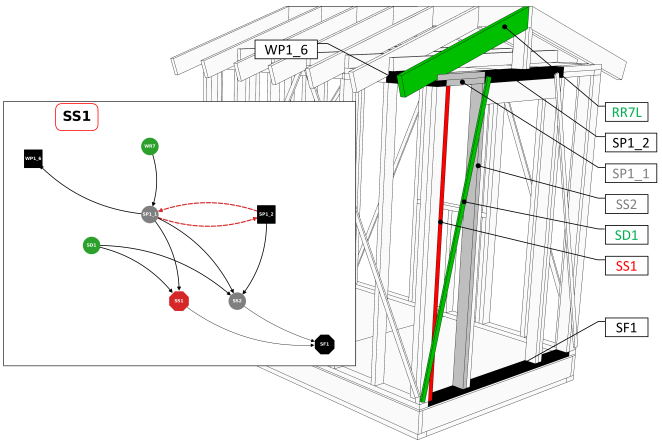
\includegraphics [trim={0cm 0cm 0cm 0cm}, clip, width=0.99\textwidth]{fig11_SS1_structure}
            \caption{active member subgraph for member SS1}
            \label{fig:fig11_ss1_a} 
    	\end{subfigure}
        %
    	\begin{subfigure}[b]{0.49\linewidth}
            \centering
            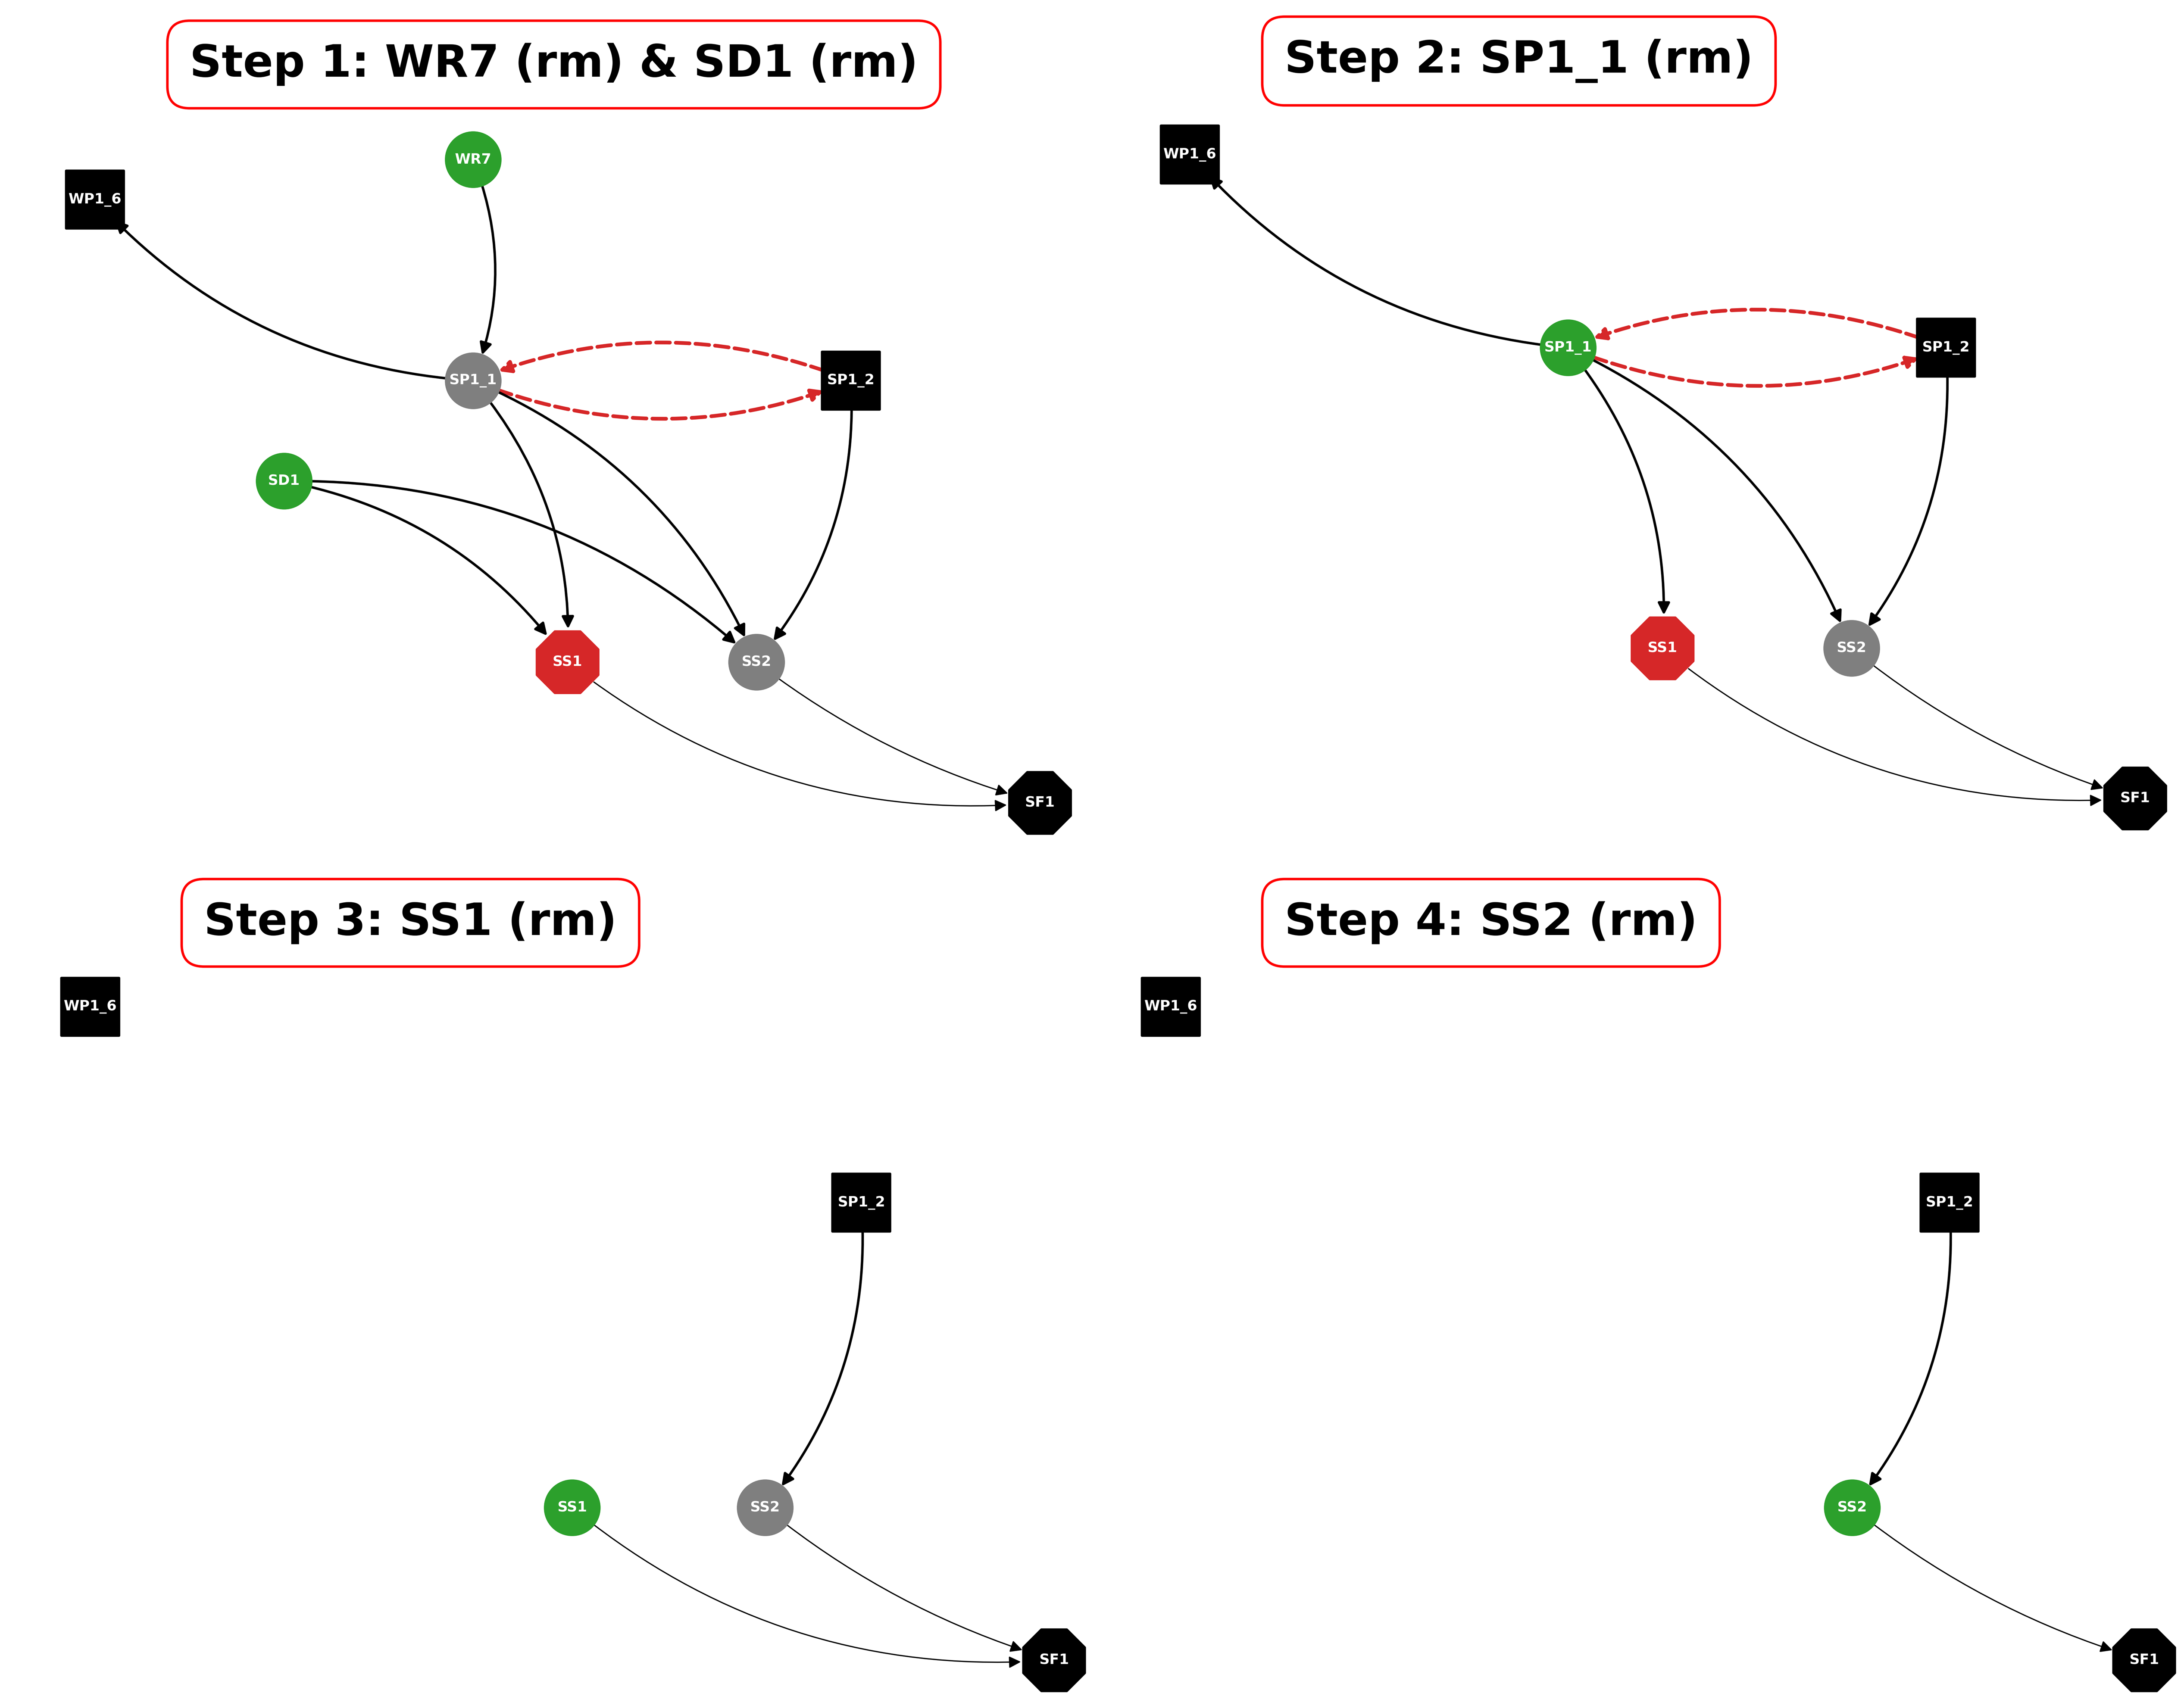
\includegraphics [trim={0cm 0cm 0cm 0cm}, clip, width=0.99\textwidth]{fig11_SS1_sequence}
            \caption{potential disassembly sequence}
            \label{fig:fig11_ss1_b} 
    	\end{subfigure}
        %
    	\caption{Planning the removal of member SS1}
    \end{figure}

    A potential four-step disassembly sequence generated from this subgraph is shown in \Cref{fig:fig11_ss1_b}. The structural and robotic kinematic feasibility evaluation reveals that the sequence is structurally feasible but fails since no robot can reach member SS1 without colliding with either member WS9 or SS3 in its path. Thus, this first iteration indicates that the removal of either WS9 or SS3 must first occur as part of the overall fabrication task. This results in the generation of two new subgraphs representing the affected region of the structure when either of these members is added as an active member.
    
    In \Cref{fig:fig12_ss1_sequences_option1}, the subgraph for option 1 is presented, involving the removal of SS3 before SS1. This option requires the removal of a total of 9 members but leads to inadequate support for member SP1\_2 upon the termination of the sequence. On the other hand, \Cref{fig:fig12_ss1_sequences_option2} depicts the subgraph for option 2, removing WS9 before SS1. Despite a more extensive removal process involving 12 members, this option ensures a stable structure at the end of the sequence. Consequently, option 2 is chosen for P1.

    \begin{figure}[ht]
    	\centering
    	\begin{subfigure}[b]{0.80\linewidth}
            \centering
            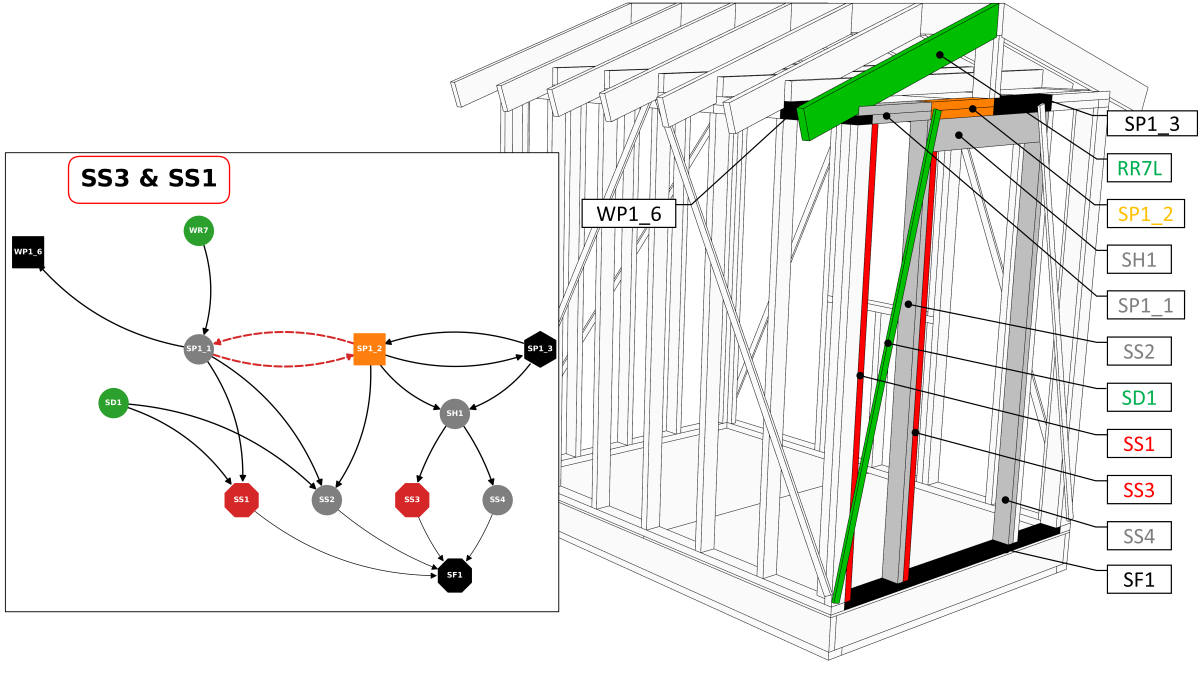
\includegraphics [trim={0cm 0cm 0cm 0cm}, clip, width=0.99\textwidth]{fig12_phase1_option2}
            \caption{option 1: adding SS3}
            \label{fig:fig12_ss1_sequences_option1} 
    	\end{subfigure}
        
    	\begin{subfigure}[b]{0.80\linewidth}
            \centering
            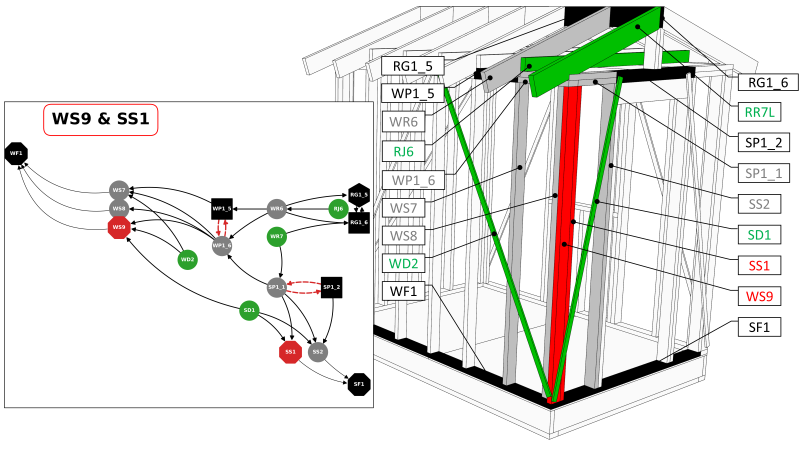
\includegraphics [trim={0cm 0cm 0cm 0cm}, clip, width=0.99\textwidth]{fig12_phase1_option1}
            \caption{option 2: adding WS9}
            \label{fig:fig12_ss1_sequences_option2} 
    	\end{subfigure}
        %
    	\caption{Two new active member subgraphs generated from the inclusion of additional removal targets determined by the feasibility evaluation for the planned removal of SS1.}
    	\label{fig:fig12_ss1_sequences} 
    \end{figure}



\subsubsection{Fabrication Sequence}
    \begin{figure}[ht]
    	\centering
    	\begin{subfigure}[b]{0.49\linewidth}
            \centering
            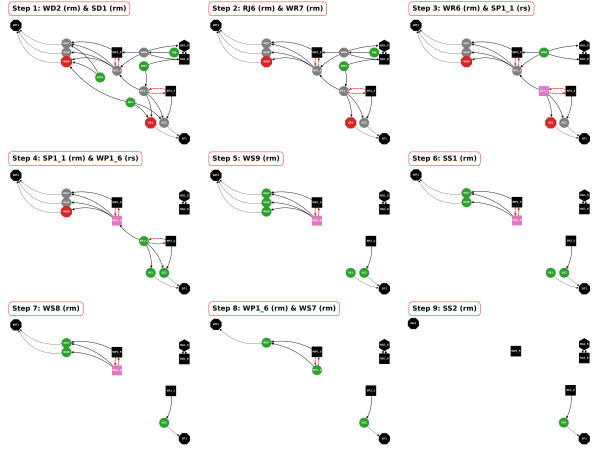
\includegraphics [trim={0cm 0cm 0cm 0cm}, clip, width=0.99\linewidth]{fig13_phase1_sequence_graph}
            \caption{sequence subgraphs}
            \label{fig:fig13_ws9_ss1_graph} 
    	\end{subfigure}
        %
        
    	\begin{subfigure}[b]{0.49\linewidth}
            \centering
            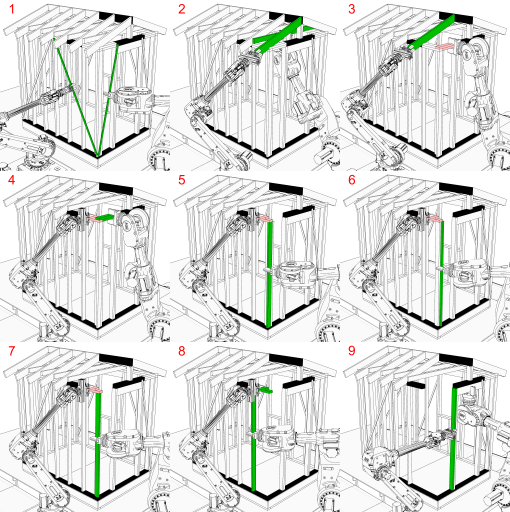
\includegraphics [trim={0cm 0cm 0cm 0cm}, clip, width=0.99\linewidth]{fig13_phase1_sequence_render}
            \caption{sequence renderings}
            \label{fig:fig13_ws9_ss1_render}
    	\end{subfigure}

    	\caption{Phase 1 disassembly sequence.}
    	\label{fig:fig13_ws9_ss1} 
    \end{figure}
    
    Assuming the availability of two robotic agents for executing the planned fabrication task, a viable disassembly sequence is derived from the active member subgraph generated for option 2 (members WS9 and SS1). This computed disassembly sequence encompasses 9 discrete steps, wherein one or two members in the subgraph are safely removed from the structure using robotic agents. The actions in each step are determined based on the current state of the structure, visually represented by an updating subgraph at each step. The progression of the sequence and the planned action at each specific step is illustrated in \Cref{fig:fig13_ws9_ss1_graph}. Simultaneously, renderings of the structure, highlighting the targeted members for removal/support at that step and depicting the robots in the correct position for execution, are presented in \Cref{fig:fig13_ws9_ss1_render}. In these figures, the pink denotes members that are temporarily physically supported by a robot, ensuring adequate stability during that step.

\subsubsection{Execution and Resulting Structure}
    The resulting structure after the completion of this 9-step disassembly sequence is displayed in \Cref{fig:fig13_ws9_ss1_final}. Further snapshots of the structure and robots at various stages of the phase are provided in \Cref{sec:appendixb_1}.

    \begin{figure}[ht]
        \centering
        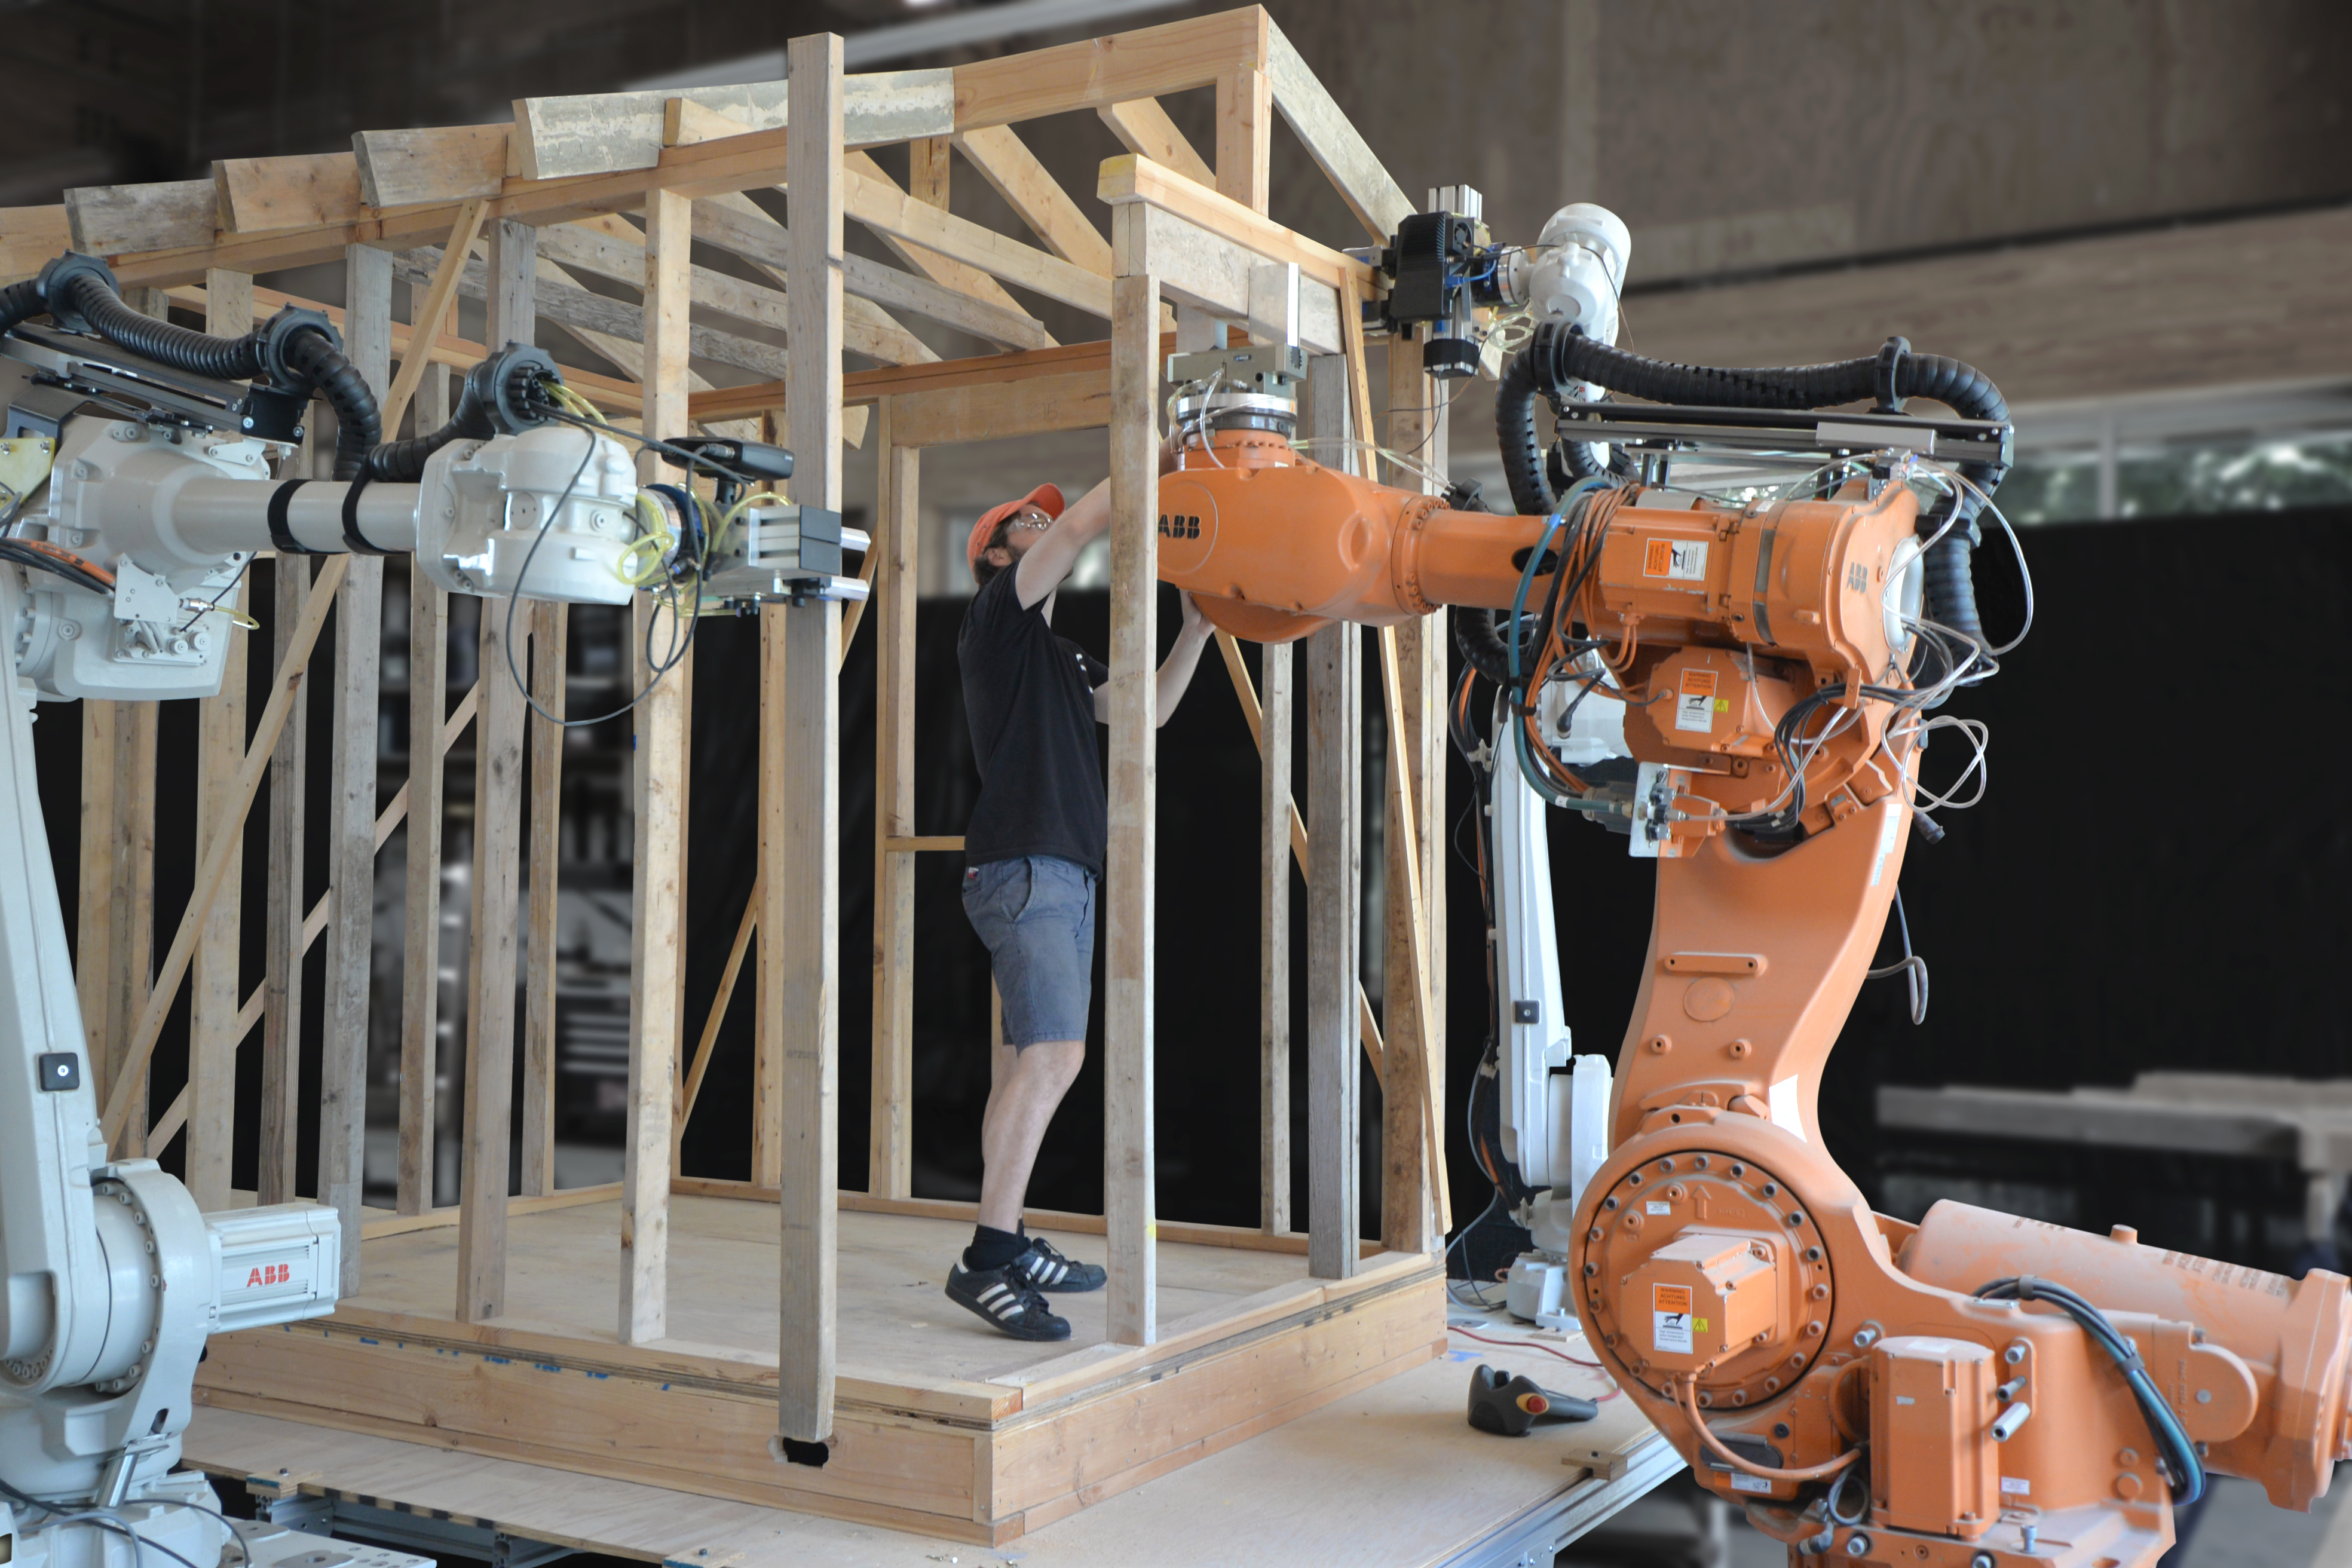
\includegraphics [trim={0cm 0cm 0cm 0cm}, clip, width=0.99\linewidth]{fig14_phase1_final_structure}
        \caption{Prototype structure at the end of the disassembly in Phase 1 (from \cite{bruun_zerowaste_2022}).}
        \label{fig:fig13_ws9_ss1_final}
    \end{figure}
    
%%%%%%%%%%%%%%%%%%%%%%%%%%%%%%%%%%%%%%%%%%%%%%%%
%%%%%%%%%%%%%%%%%%%%%%%%%%%%%%%%%%%%%%%%%%%%%%%%
%%%%%%%%%%%%%%%%%%%%%%%%%%%%%%%%%%%%%%%%%%%%%%%%
\newpage
\subsection{Phase 2 (P2): Full Wall Disassembly and Partial Reassembly}
    Building upon the methodologies explored in the initial phase, the second phase of the study extends the disassembly goal beyond a single-member target, as seen in P1. In P2, the objective is to safely remove a larger and more geometrically complex portion of the remaining South wall of the structure. This phase also introduces increased complexity in robotic planning by engaging all three available robots throughout the planned sequence.
    
    In P2 the scope of the overall fabrication process is broadened by incorporating structural reassembly after completing the disassembly phase. This serves as a practical test for the reuse of members removed from the structure for alternative purposes. The disassembly goal in P2 is meant to explore what can be done when achieving a structurally sound final structure after disassembly is not possible without external support. Unlike P1, where a small disassembly intervention meant that finding a feasible sequence resulting in a stable final structure was possible, P2 involves a much larger and more complex disassembly operation where no safe resulting structure is identified within reasonable constraints (i.e., without calculating a sequence to dismantle the entire structure).
    
    Thus, following the completion of disassembly in P2, the only viable means to safely conclude the process is either to provide external temporary support structures at the targeted location or to reuse several removed members to reassemble a new but simple supporting structure. Notably, this reassembly is considered partial, meaning that not all initially removed members are incorporated into the new structure. Additionally, in P2, the specific configuration of the new structure is not optimized; it solely acts as a prop, providing basic structural support to a region of the structure deemed unsafe after the disassembly is completed.

\subsubsection{Preliminary Planning}
    To facilitate the removal of the entire South wall, the members chosen include the remaining top plate members SP1\_2, SP1\_3, and SP1\_4. This selection forms the disassembly subgraph depicted in \Cref{fig:fig15_p2_planning_a}. Like the preceding phase (P1), the resultant disassembly sequence proves infeasible due to unavoidable collisions, particularly with member ES10. To address this challenge, as illustrated in \Cref{fig:fig15_p2_planning_b}, ES10 is incorporated as a removal target prior to dismantling the top plate. However, this adjustment also yields an unsatisfactory sequence, revealing inadequate support for the ridge beam member RG1\_6 upon completion of the disassembly process.
    
    To rectify this structural instability, RG1\_6 is included in the disassembly sequence, leading to the configuration shown in \Cref{fig:fig15_p2_planning_c}. Yet, the removal of RG1\_6 fails to resolve the issue, as the instability concern is transferred to the subsequent member, RG1\_5. Upon further examination, it becomes evident that achieving stability necessitates the removal of the entire ridge beam, along with all roof girders and joists. However, such an extensive intervention exceeds the intended scope of disassembly. Consequently, the disassembly process is limited to the members highlighted in the structure as shown in \Cref{fig:fig15_p2_planning_c}, requiring a subsequent reassembly phase with additional support provided to stabilize member RG1\_5 at the conclusion of the sequence.


    \begin{figure}[ht]
    	\centering
    	\begin{subfigure}[b]{0.45\linewidth}
            \centering
            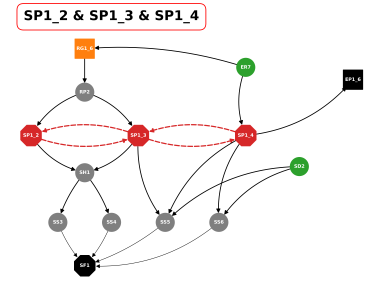
\includegraphics [trim={0cm 0cm 0cm 0cm}, clip, width=0.99\textwidth]{fig15_phase2_option1}
            \caption{removing top plate.}
            \label{fig:fig15_p2_planning_a} 
    	\end{subfigure}
        %
    	\begin{subfigure}[b]{0.45\linewidth}
            \centering
            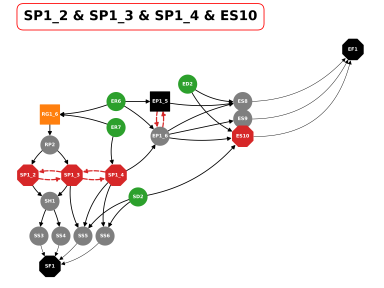
\includegraphics [trim={0cm 0cm 0cm 0cm}, clip, width=0.99\textwidth]{fig15_phase2_option2}
            \caption{adding member ES10.}
            \label{fig:fig15_p2_planning_b} 
    	\end{subfigure}
        %
        
    	\begin{subfigure}[b]{0.90\linewidth}
            \centering
            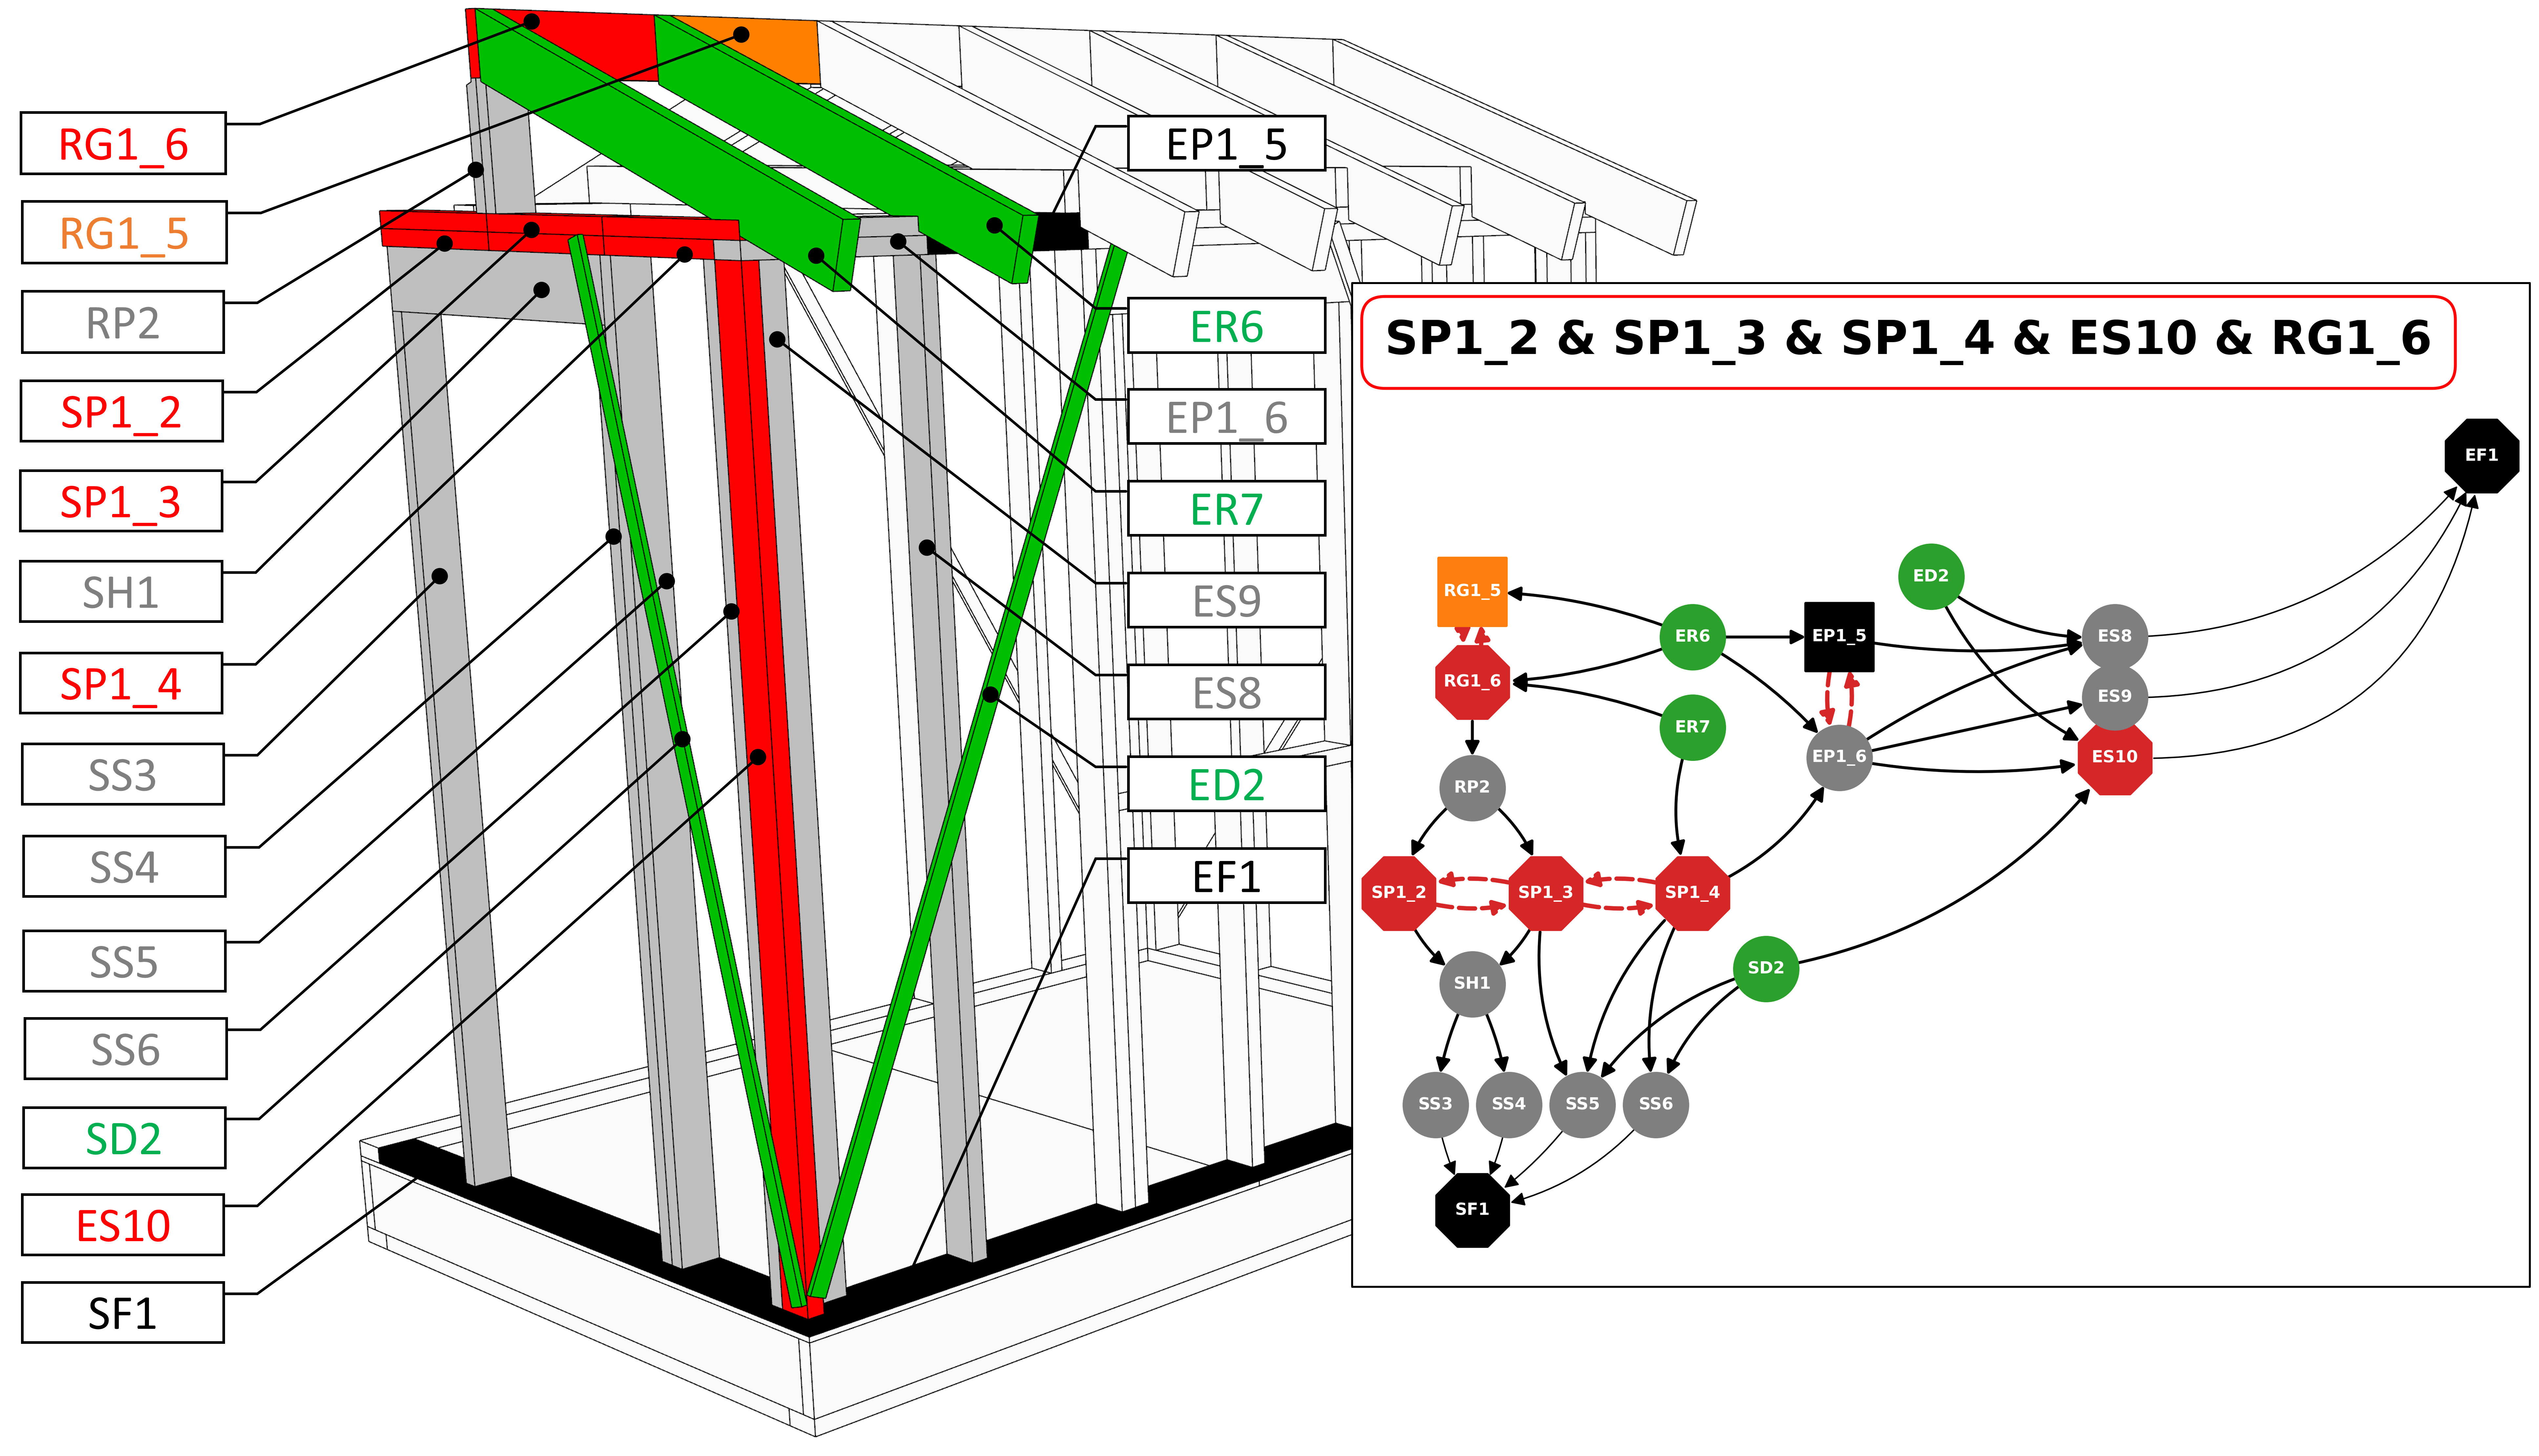
\includegraphics [trim={0cm 0cm 0cm 0cm}, clip, width=0.99\textwidth]{fig15_phase2_option3}
            \caption{final disassembly subgraph when adding RG1\_6.}
            \label{fig:fig15_p2_planning_c} 
    	\end{subfigure}
        %
    	\caption{Planning the removal of the south wall as part of Phase 2 and resulting in a final structure that requires additional support.}
    	\label{fig:fig15_p2_planning} 
    \end{figure}


\subsubsection{Fabrication Sequence}
    Assuming the availability of all three robotic agents for executing the planned fabrication task, a viable disassembly sequence is calculated for the disassembly subgraph shown in \Cref{fig:fig15_p2_planning_c}. The progression of the sequence and the planned action at each specific step is illustrated in \Cref{fig:fig16_p2_sequence_graph}. Simultaneously, renderings of the structure, highlighting the targeted members for removal/support at that step and depicting the robots in the correct position for execution, are presented in \Cref{fig:fig16_p2_sequence_render}. In these figures, the pink denotes members that are temporarily physically supported by a robot, ensuring adequate stability during that step.

    \begin{figure}[ht]
    	\centering
    	\begin{subfigure}[b]{0.49\linewidth}
            \centering
            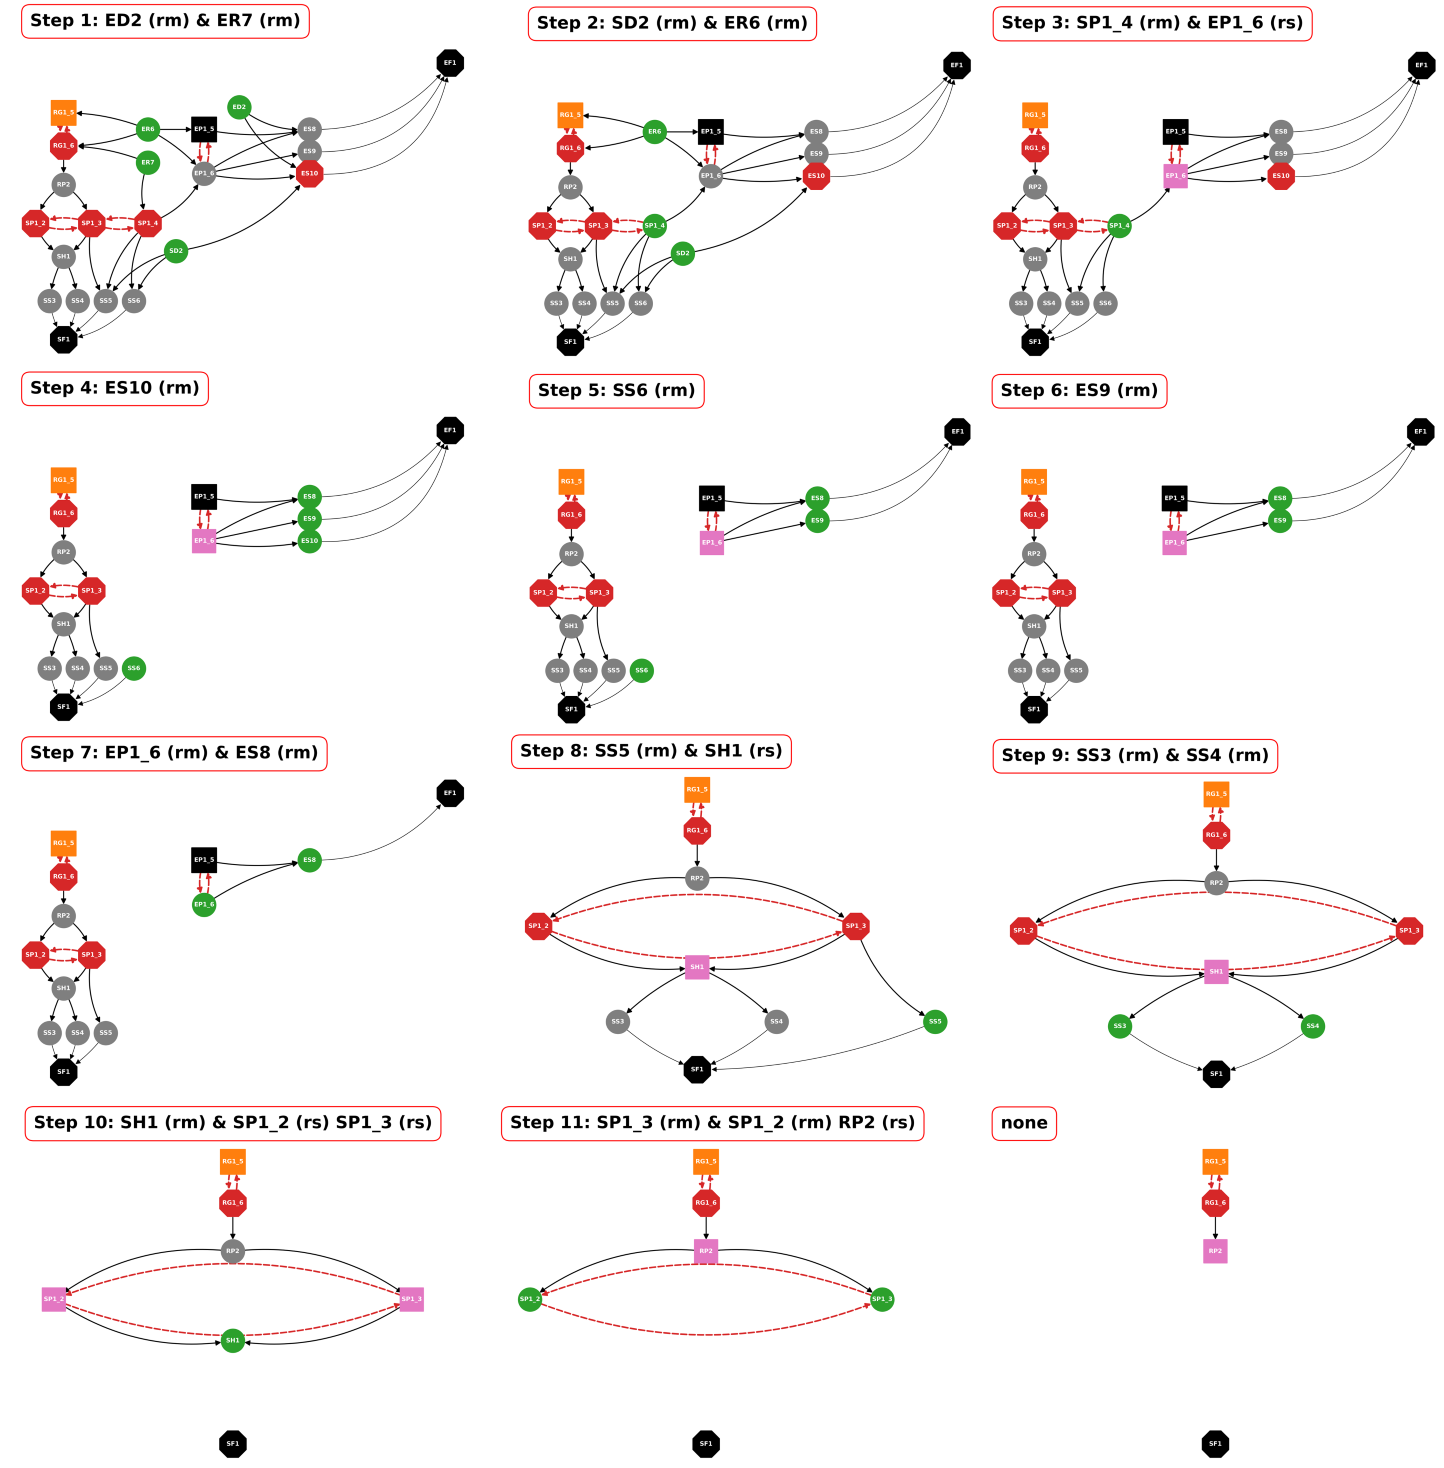
\includegraphics [trim={0cm 0cm 0cm 0cm}, clip, width=0.99\linewidth]{fig16_phase2a_sequence_graph}
            
            \caption{sequence subgraphs}
            \label{fig:fig16_p2_sequence_graph}
    	\end{subfigure}
        %
    	\begin{subfigure}[b]{0.49\linewidth}
            \centering
            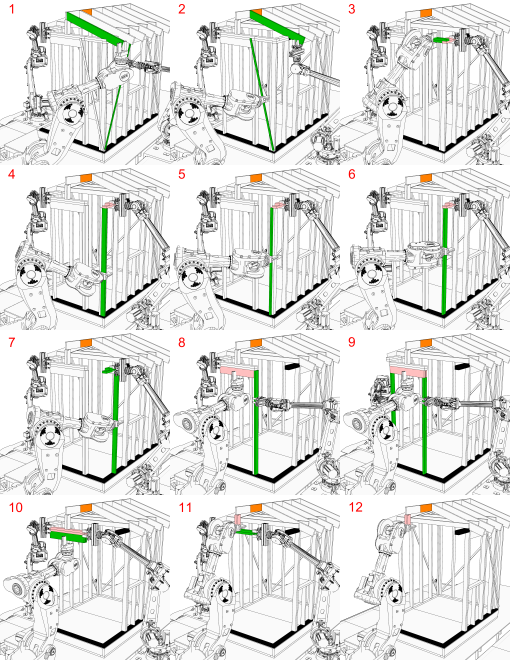
\includegraphics [trim={0cm 0cm 0cm 0cm}, clip, width=0.99\linewidth]{fig16_phase2a_sequence_render}
            \caption{sequence renderings}
            \label{fig:fig16_p2_sequence_render}
    	\end{subfigure}
    	\caption{Phase 2 disassembly sequence.}
    	\label{fig:fig16_p2_sequence} 
    \end{figure}

    The disassembly sequence unfolds through steps 1 to 8, reminiscent of P1, employing only two robots. However, from step 9 onwards, the involvement of all three robots becomes necessary, orchestrating a leapfrogging strategy to dismantle the members supporting the roof girder. In step 12 the structure is shown in its temporary state, stabilized by R3. At this point, further disassembly is hindered, given that only R3 can access the final members but R3 must concurrently support the structure at this step. In addition, RG1\_5 will eventually require additional support at the conclusion of the disassembly as noted when planning this sequence. To address both challenges, a reassembly stage is initiated after step 12. 

    Several recently removed members — namely ER6, ER7, SS6, SS4, and SS4 — are strategically reassembled into a new supporting structure as shown in steps 13 to 17 in \Cref{fig:fig17_p2_sequence}. This new structure not only provides crucial support to member RG1\_5 but also frees R3 since it is no longer required for support and can thus continue with the remaining disassembly steps. The final members are removed by R3 in steps 17 and 18, completing the planned disassembly sequence while resulting in a structurally sound final configuration.

    \begin{figure}[ht]
    	\centering
    	\begin{subfigure}[b]{0.70\linewidth}
            \centering
            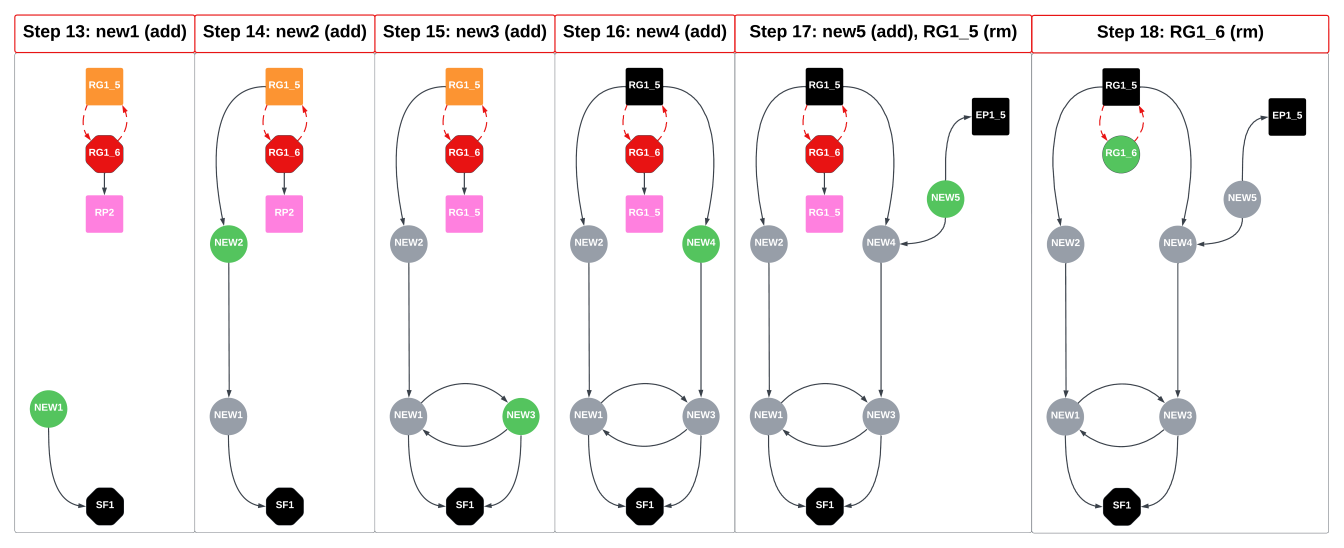
\includegraphics [trim={0cm 0cm 0cm 0cm}, clip, width=0.99\textwidth]{fig17_phase2b_sequence_graph}
            \caption{sequence subgraphs}
    	\end{subfigure}
        %
        
    	\begin{subfigure}[b]{0.70\linewidth}
            \centering
            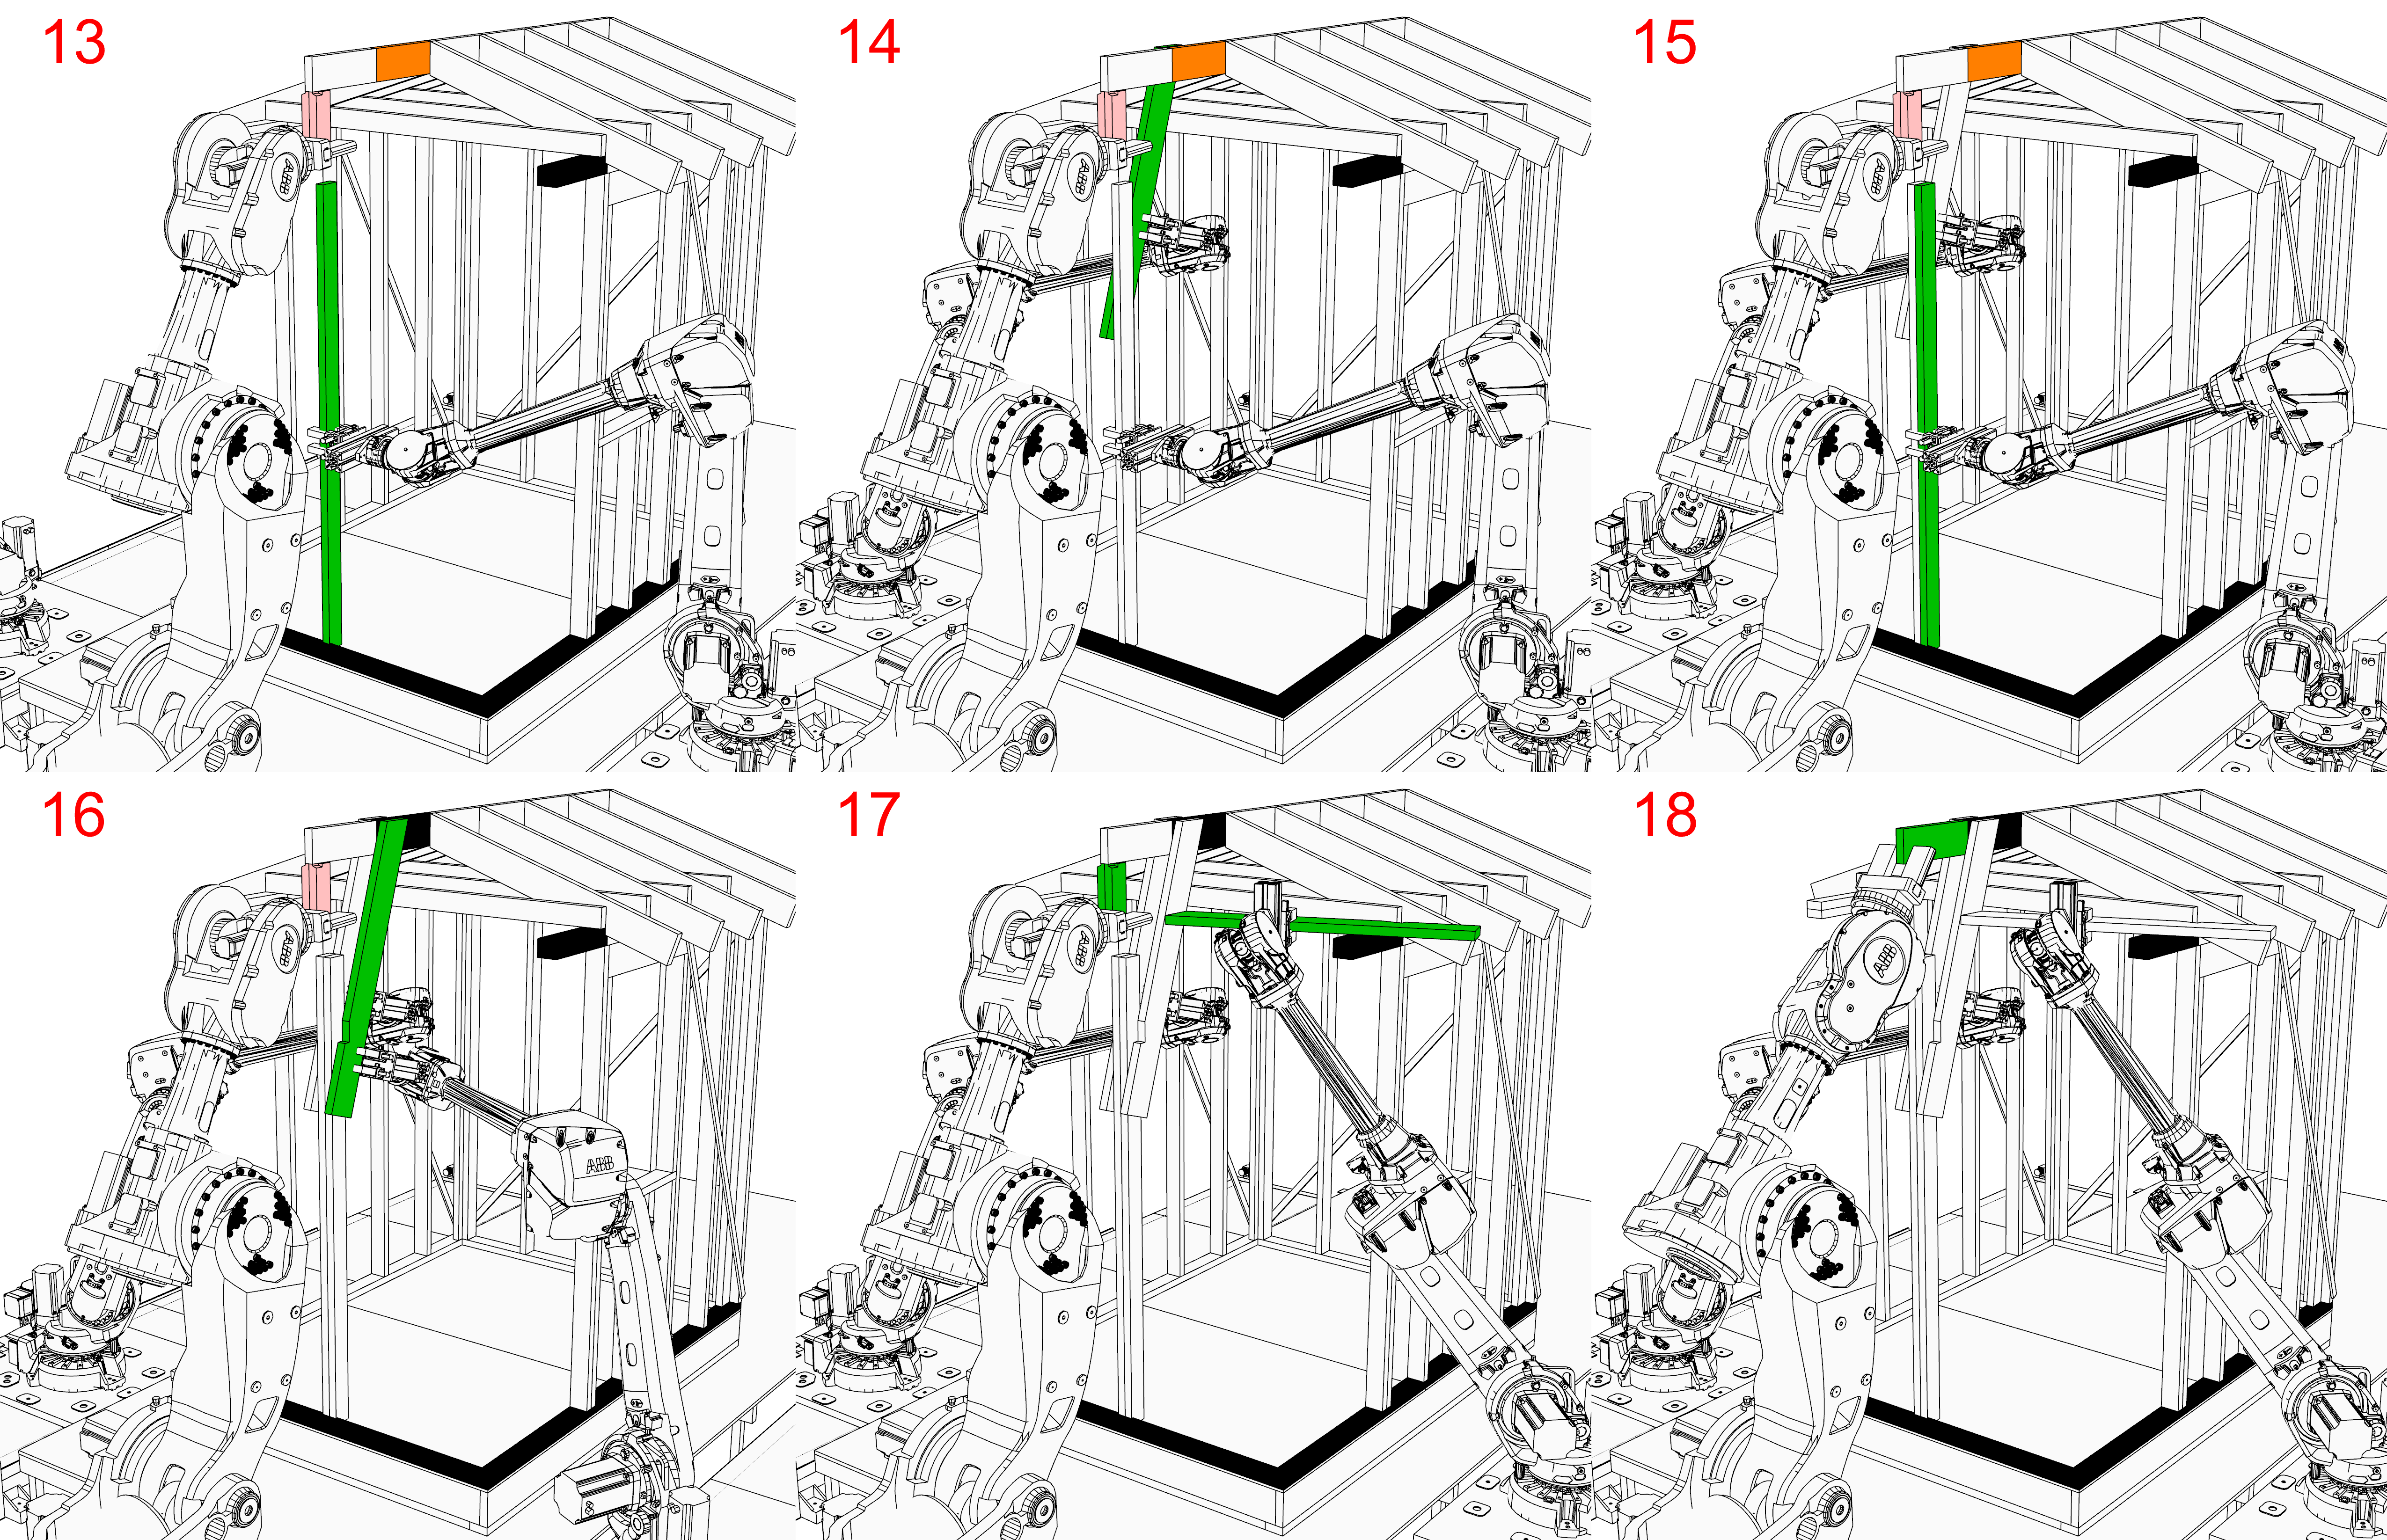
\includegraphics [trim={0cm 0cm 0cm 0cm}, clip, width=0.99\textwidth]{fig17_phase2b_sequence_render}
            \caption{sequence renderings}
    	\end{subfigure}
    	\caption{Phase 2 reassembly sequence.}
    	\label{fig:fig17_p2_sequence} 
    \end{figure}

\subsubsection{Execution and Resulting Structure}
    \Cref{fig:fig18_p2_disassembly} shows snapshots of the disassembly sequence at two critical steps. In step 10, all three robots are required. In step 12, R3 is used to support the roof girder before the reassembly begins and additional support is added to the structure.

    \begin{figure}[ht]
        \centering
        \begin{subfigure}[b]{0.49\linewidth}
            \centering
            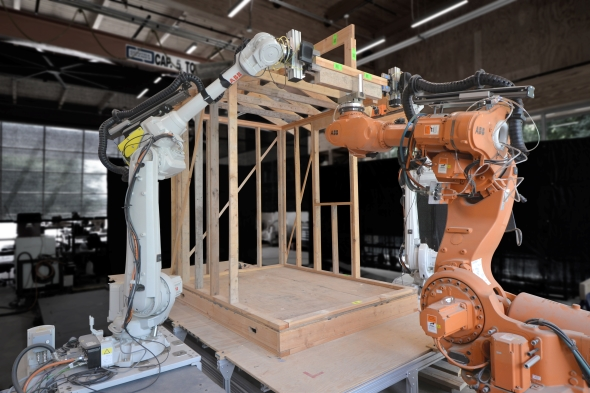
\includegraphics [trim={0cm 0cm 0cm 0cm}, clip,  height=5.2cm]{fig18_phase2_step10}
            \caption{Step 10 in the disassembly sequence. R3 is ready to remove SH1, while R1 and R2 support SP1\_2 and SP1\_3 respectively (from \cite{bruun_cooperative_2024}).}
        \end{subfigure}
        %
        \begin{subfigure}[b]{0.49\linewidth}
            \centering
            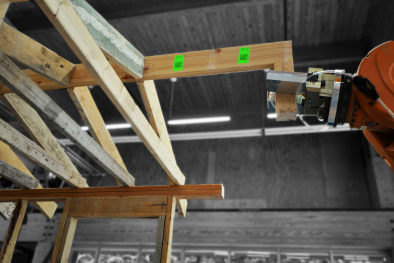
\includegraphics [trim={0cm 0cm 0cm 0cm}, clip,  height=5.2cm]{fig18_phase2_step12}
            \caption{Step 12 in the disassembly sequence. R3 is supporting the remaining roof structure before the start of the reassembly sequence.}
        \end{subfigure}
    	\caption{Snapshots of Phase 2 disassembly.}
    	\label{fig:fig18_p2_disassembly} 
    \end{figure}

    \begin{figure}[ht]
        \centering
        \begin{subfigure}[b]{0.49\linewidth}
            \centering
            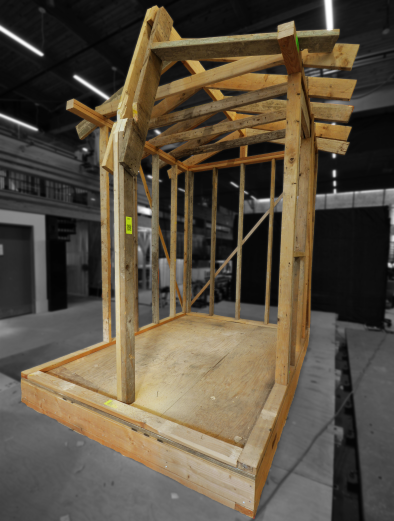
\includegraphics [trim={0cm 0cm 0cm 0cm}, clip, height=10.5cm]{fig19_phase2_final_structure}
            \caption{Prototype structure.}
            \label{fig:fig19a_p2_final}
        \end{subfigure}
        %
        \begin{subfigure}[b]{0.49\linewidth}
            \centering
            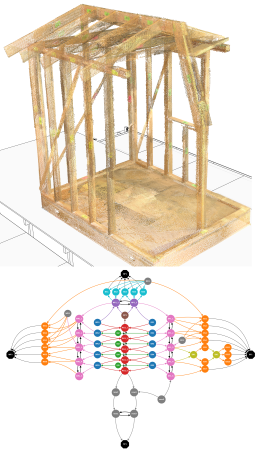
\includegraphics [trim={0cm 0cm 0cm 0cm}, clip, height=10.5cm]{fig19_phase3_start}
            \caption{As-built pointcloud \& assembly hierarchy.}
            \label{fig:fig19b_p2_final}
        \end{subfigure}
        \caption{The prototype structure at the end of the disassembly and reassembly in Phase 2.}
    \end{figure}

    The completed structure resulting from the reassembly sequence is shown in \Cref{fig:fig19a_p2_final}. Additional snapshots illustrating various steps during disassembly and reassembly are presented in \Cref{sec:appendixb_2}. Upon concluding Phase 2, in preparation for subsequent phases, the point cloud gathering procedure outlined in \Cref{sec:4a_camera} is repeated to capture deformations in the structure and the as-built position of the newly added members. This updated point cloud and the assembly hierarchy graph are shown in \Cref{fig:fig19b_p2_final}.




%%%%%%%%%%%%%%%%%%%%%%%%%%%%%%%%%%%%%%%%%%%%%%%%
%%%%%%%%%%%%%%%%%%%%%%%%%%%%%%%%%%%%%%%%%%%%%%%%
%%%%%%%%%%%%%%%%%%%%%%%%%%%%%%%%%%%%%%%%%%%%%%%%
\clearpage
\subsection{Phase 3 (P3): Full Wall and Roof Disassembly and Reassembly}
    
   Phase 3 marks the project's culmination, surpassing the disassembly scopes of P1 and P2. In P3 the objective is to remove all remaining members in the West wall and roof sub-structures. Additionally, it introduces tighter constraints in reassembly, adopting a one-to-one approach: each extracted member is reincorporated to reshape the West wall into a lattice structure, improving its overall lateral stiffness.

\subsubsection{Preliminary Planning}
    As illustrated in \Cref{fig:fig20_p3_planning}, Phase 3 designates twelve remaining members within the West wall and roof sub-structures for removal. The diagonal brace (WD1), is also planned for removal, but is not considered a valid member for reuse since the diagonal members take the place of typical planar sheathing used to provide lateral stiffness.
    
    Only the two stud members in the North corner (WS1 and WS2) and the top plate (WP1) are not specified as removal targets. Retaining the corner stud members prevents the need to extend the disassembly sequence into the North wall, while the top plate acts as a support constraint for the newly reassembled wall. The planned goal for the reassembly process in P3 is to fit the new lattice wall structure within the current volume of the existing wall. This means that all the new members must fit within the original 4" thickness specified by the stud members in the wall (i.e., for a 2x4" stud wall).

    \begin{figure}[ht]
        \centering
        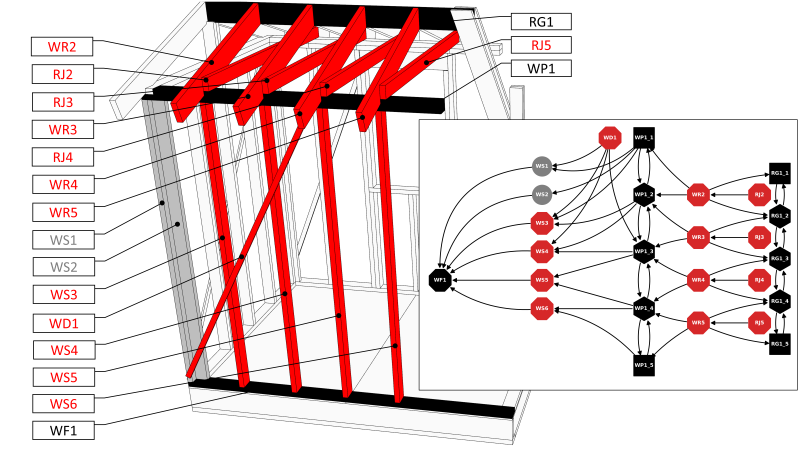
\includegraphics [trim={0cm 0cm 0cm 0cm}, clip, width=0.99\linewidth]{fig20_phase3_planning}
        \caption{The disassembly subgraph for the removal of the West wall and roof members.}
        \label{fig:fig20_p3_planning}
    \end{figure}

\subsubsection{Fabrication Sequence}
    The disassembly and reassembly of the twelve specified target members results in a fabrication sequence consisting of 25 steps. This sequence can be represented as two distinct sub-tasks: (1) Steps 1-12 involve the removal and reassembly of the initial set of 6 members, while (2) Steps 14-25 pertain to the removal and reassembly of the subsequent set of 6 members. The first set consists of disassembling and reassembling members WS6, RJ5, WR5, RJ4, WR4, and WS5 (in order) and the second set consists of disassembling and reassembling members RJ3, WR3, WS4, RJ2, WR2, WS3 (in order). 
    
    In \Cref{fig:fig21_p3_sequence}, the planned fabrication sequence is shown as a series of renderings of the structure at each step, highlighting the remaining members in the structure still requiring removal/support, the newly placed members, and the position of the robots involved in each step. Upon reassembly into the structure, the members are depicted in white, signifying that they are no longer part of the active sequence plan. To streamline the presentation within the main body of the chapter, the corresponding support hierarchy subgraphs for each step are provided in \Cref{sec:appendixb_3}. Step 13, which is omitted from \Cref{fig:fig21_p3_sequence}, represents the removal of the diagonal member (WD1), which as previously established is just a placeholder element used in lieu of planar sheathing. In both the renderings and subgraphs, the pink denotes members temporarily supported by a robot, providing the necessary stability during the execution of the sequence.


    \begin{figure}[H]
        \centering
        \begin{subfigure}{0.95\linewidth}
            \centering
            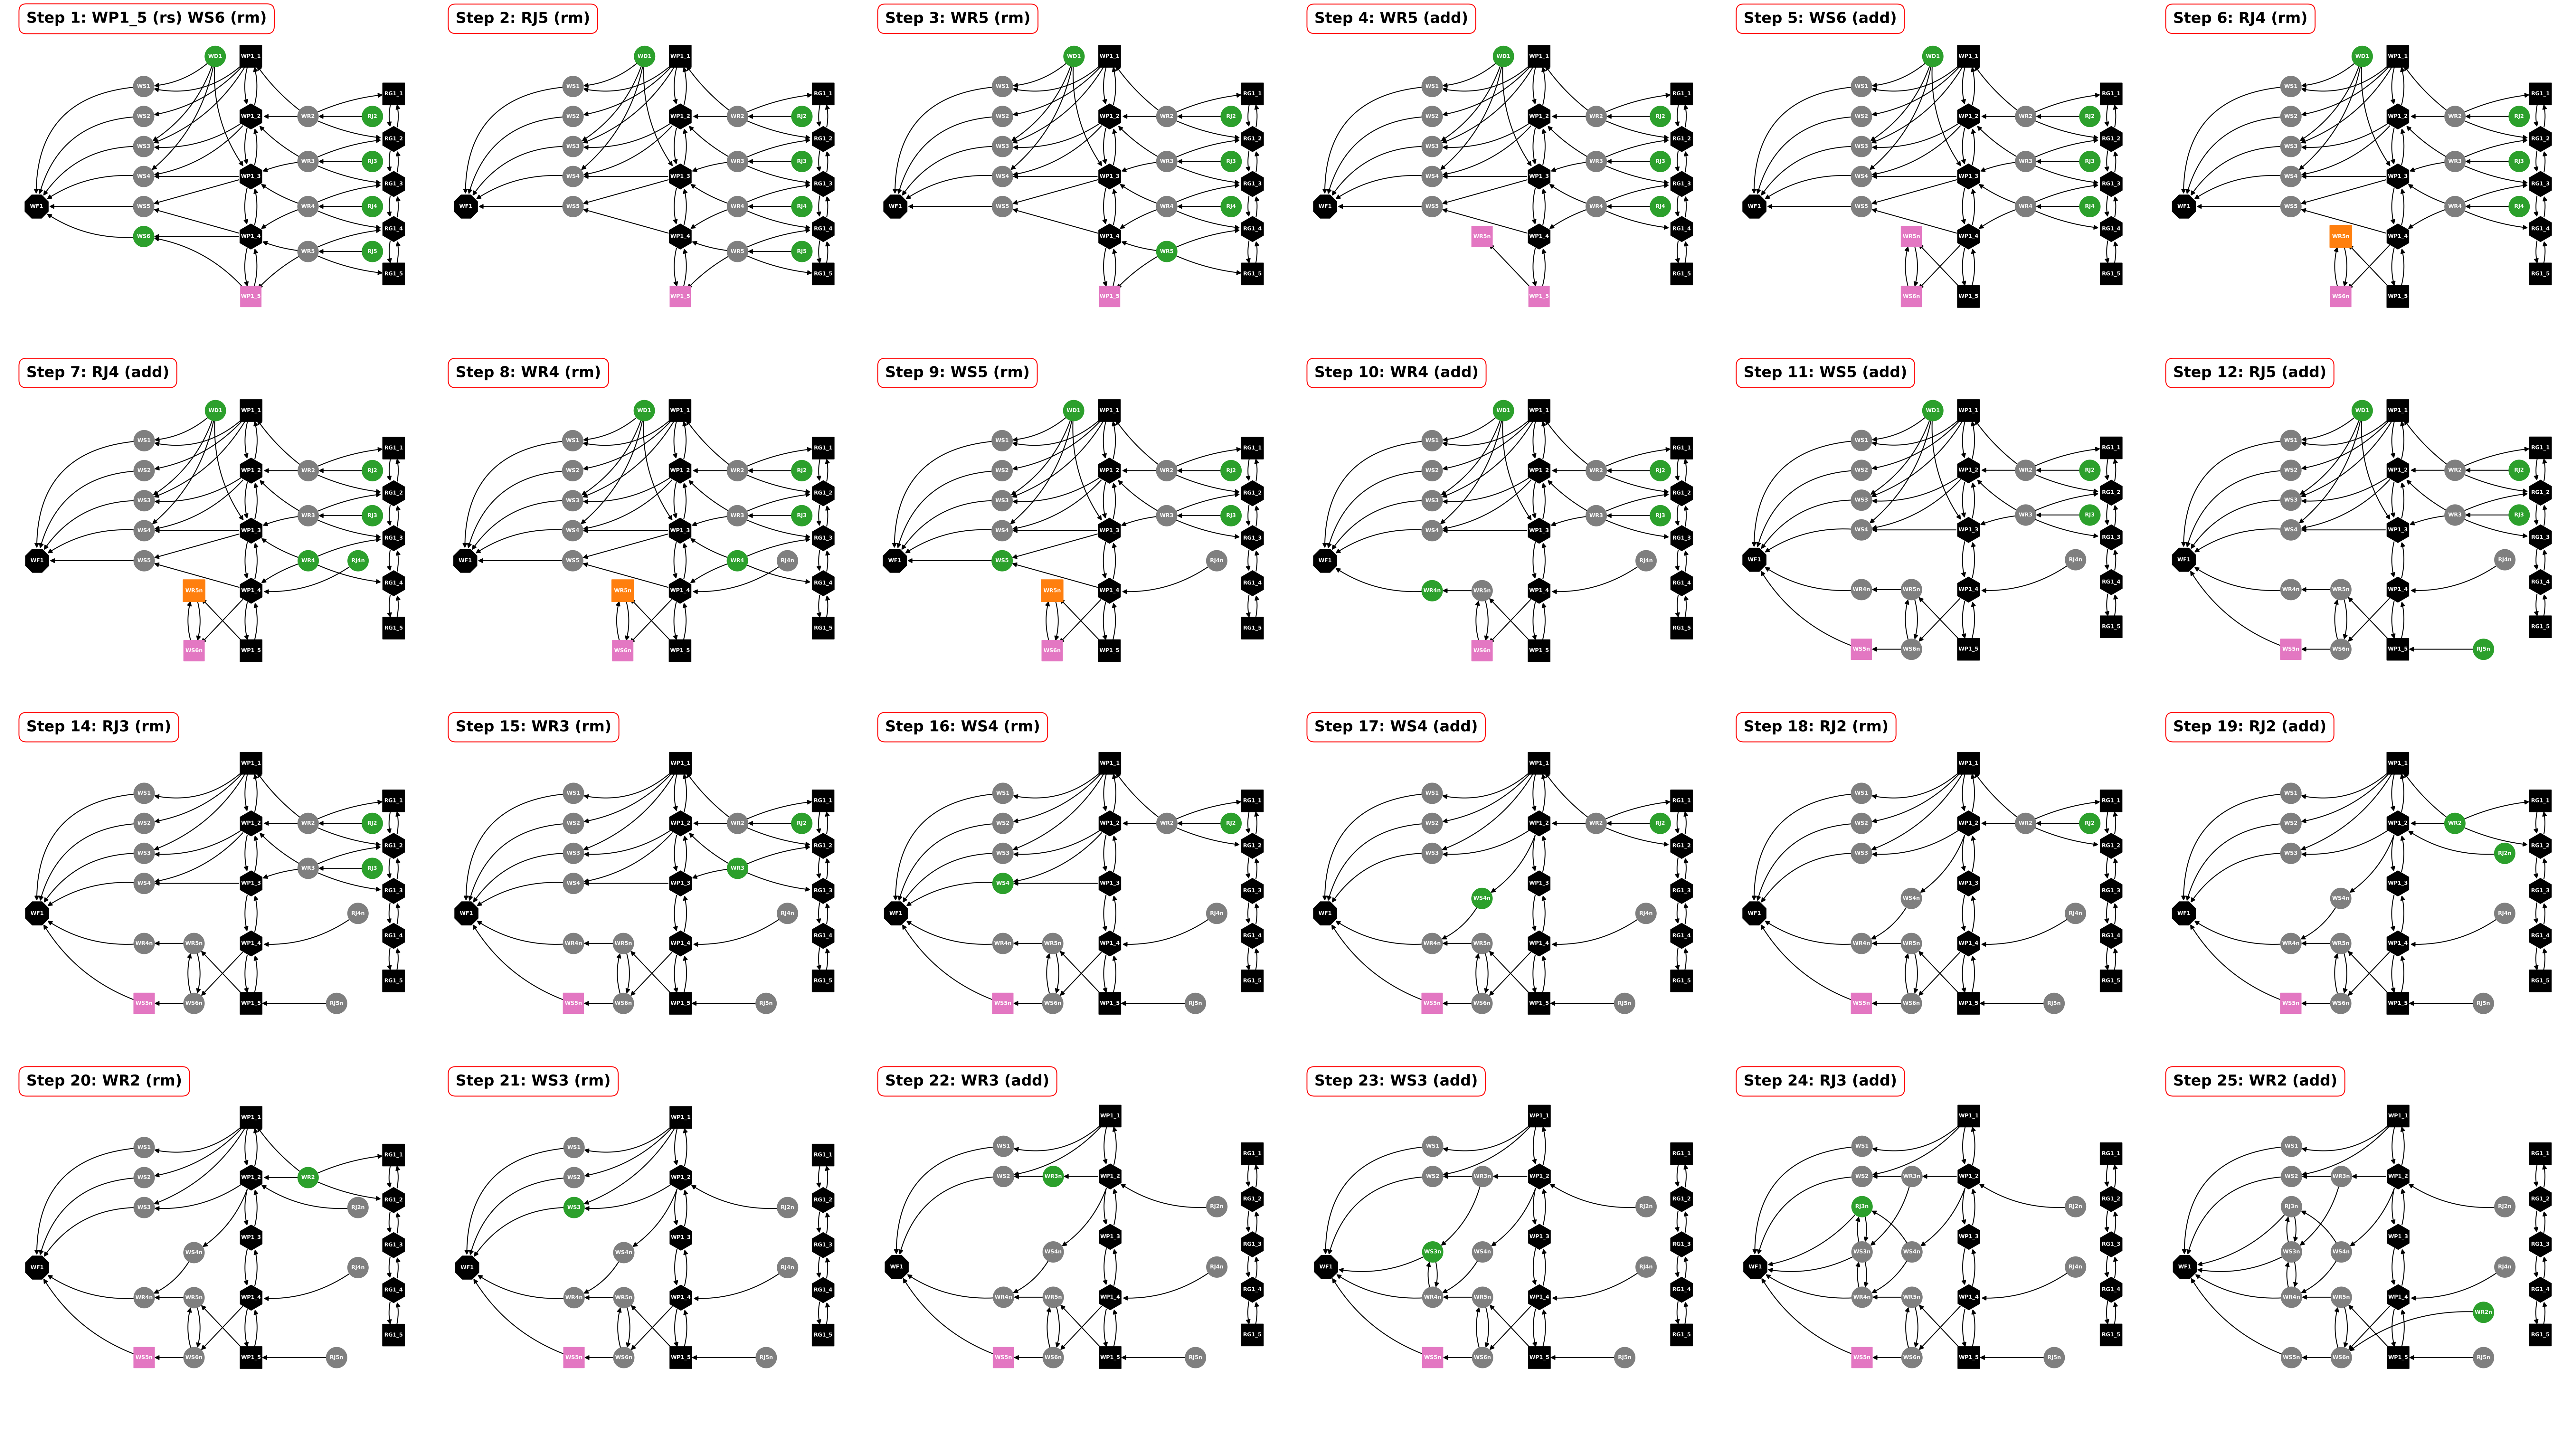
\includegraphics [trim={0cm 0cm 0cm 0cm}, clip, width=0.99\linewidth]{fig99_appendix_phase3_1}
            \caption{sequence subgraphs}
        \end{subfigure}
        %
        \vspace{5mm}
        
        \begin{subfigure}{0.95\linewidth}
            \centering
            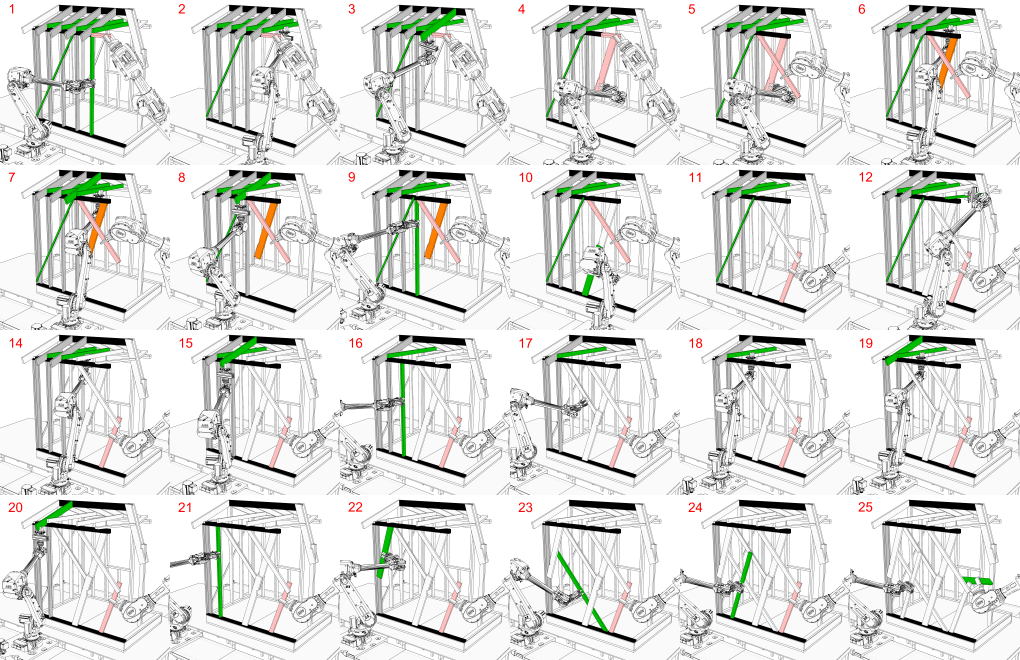
\includegraphics [trim={0cm 0cm 0cm 0cm}, clip, width=0.99\linewidth]{fig21_phase3_sequence_render}
            \caption{sequence renderings}
        \end{subfigure}
        \caption{Phase 3 disassembly and full reassembly (each member removed is reused).}
        \label{fig:fig21_p3_sequence}
    \end{figure}

\newpage
\subsubsection{Execution and Resulting Structure}
    \Cref{fig:fig22a_p3_final} shows a snapshot of the newly assembled structure at the end of step 24, as R2 is positioning the final planar element into the wall. Four of the reassembled members (e.g., RJ4, RJ5, RJ2, WR2) are placed in the out-of-plane direction to provide bracing to the wall, thus the planar wall itself consists of only eight new members. As shown in \Cref{fig:fig22b_p3_final} the result is a planar wall where the standard vertical stud wall typology is replaced with a lattice typology. The lattice arrangement features members crossing at several points. At each of these points the members are connected to each other to stiffen the entire wall system. The members are arranged along their strong axis, meaning that the thickness into the plane of the wall is only 2", thus two members can cross and still fit within the original 4" wall cavity as specified by the original wall studs.

    \begin{figure}[ht]
        \centering
        \begin{subfigure}{0.59\linewidth}
            \centering
            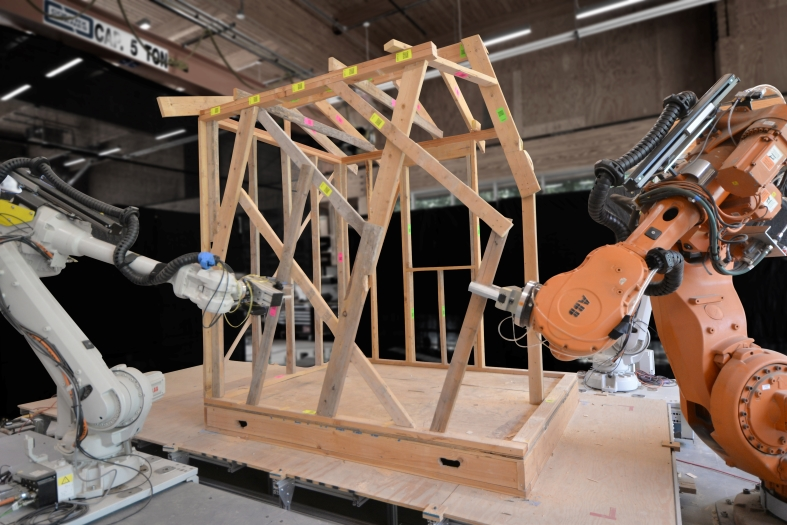
\includegraphics [trim={0cm 0cm 0cm 0cm}, clip, height=6cm]{fig22_phase_final1}
            \caption{Step 24 in the disassembly/reassembly sequence showing R2 placing the final member into the planar wall.}
            \label{fig:fig22a_p3_final} 
        \end{subfigure}
        %
        \begin{subfigure}{0.39\linewidth}
            \centering
            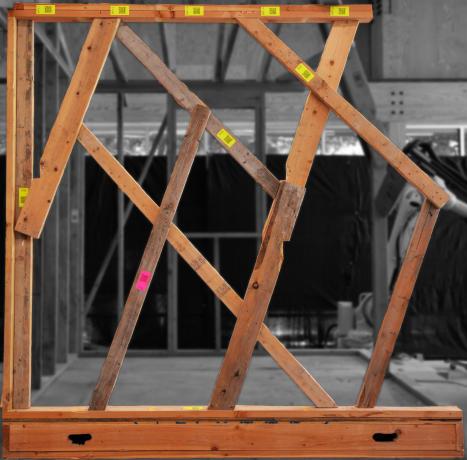
\includegraphics [trim={0cm 0cm 0cm 0cm}, clip, height=6cm]{fig22_phase_final2}
            \caption{Elevation of the finished West wall reassembled into a lattice structure.}
            \label{fig:fig22b_p3_final} 
        \end{subfigure}
        \caption{The prototype structure at the end of the disassembly and reassembly in Phase 3.}
    \end{figure}

    Two linear elastic finite element analyses were conducted to compare the relative lateral stiffness of the original and reassembled West wall. Despite the mass increasing from 34.4 to 44.1 kg between the original and reassembled wall, a significant improvement in stiffness was noted. For instance, the unbraced original wall with vertical studs exhibited a maximum deflection at its top of 67.6 cm, whereas the reassembled wall with a lattice configuration experienced a lateral deflection of only 0.3 cm. This comparison was solely intended for relative assessment, thus the applied lateral loading of 5 kN at the top of the walls was arbitrarily chosen. Additionally, to ensure comparability, identical support conditions were maintained across the models, with supports modeled as pins and connections between members fixed. Representing joints in a traditional stud wall as fixed is a conservative assumption since these connections are typically more flexible, suggesting that the actual performance of the traditional wall might be even worse if flexibility were introduced in the joints. The successful reassembly of the West wall in Phase 3 demonstrated the potential for rebuilding a structure with enhanced structural performance.

    \begin{figure}[ht]
        \centering
        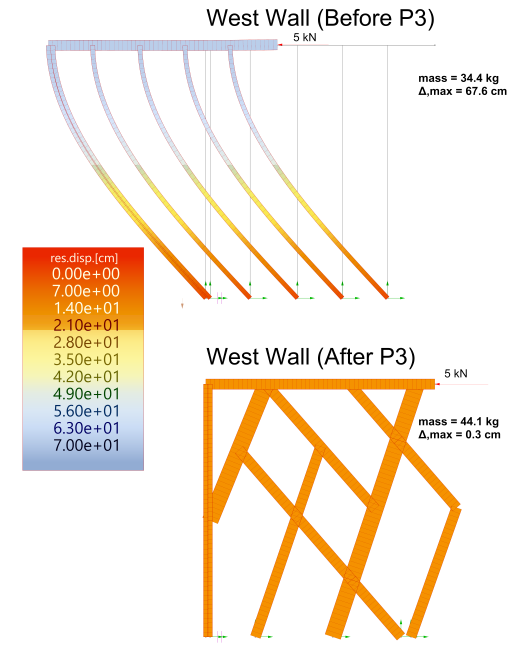
\includegraphics [trim={0cm 0cm 0cm 0cm}, clip, width=0.70\linewidth]{fig23_wall_deform}
        \caption{Finite element analysis comparing the lateral stiffness of the original (top) to the reassembled (bottom) West wall.}
        \label{fig:fig23_p3_stiffness}
    \end{figure}

    \Cref{fig:fig23_p3_stiffness} shows the results of the finite element analyses, visually depicting the relative difference in deflection between the two configurations. While conventional stud walls typically rely on planar sheathing elements for lateral stiffness, advancements in digital fabrication raise questions about the necessity of this approach. Precise placement of elements in space allows for exploration of alternative geometries beyond conventional rectilinear forms. As demonstrated by the reassembled West wall, approximately the same amount of material arranged in a planar lattice structure can effectively resist both gravity and lateral loads, thus sheathing would not be required for structural performance, potentially leading to flexibility in how such a wall unit would be designed in the future. With the growing availability of flexible robotic fabrication setups these results challenge the traditional notion that timber framing must adhere to rectilinear forms, which have been developed for ease of manual construction.




% ----------------------------------------------------------------------------------------------------
% 6. Conclusion
% ----------------------------------------------------------------------------------------------------
\section{Conclusion} \label{sec:6_conclusion}
    This chapter presented the detailed computational workflow for performing scaffold-free cooperative robotic disassembly and reassembly processes for existing timber structures as a continuation of a preliminary publication on the topic \cite{bruun_zerowaste_2022}. It demonstrated how cooperative robotic cells could be used to collect data on unknown structures while enabling the planning and execution of feasible disassembly and reassembly without requiring external scaffolding. The ZeroWaste project exemplified how material reuse, as a consideration for a circular economy, can be paired with the capabilities of contemporary cooperative robotic fabrication systems. This research has advanced sustainability and technological sophistication in the construction sector, emphasizing efficiency, resource management, and environmental stewardship.

\subsection{Summary of Results}
    The chapter first introduces the computational methods developed as part of the ZeroWaste project. These methods were subsequently applied to achieve various goals pertaining to circular economy principles and the integration of computational and cooperative robotic fabrication methods.
    
    In terms of circular economy principles, the fabrication tasks undertaken on the prototype structure demonstrated the potential for existing timber buildings to function as reservoirs for reusable materials. By employing varying levels of disassembly and reassembly on an unidentified timber prototype structure, the capacity to generate fresh structural configurations using previously utilized materials was highlighted.
    
    In terms of computational and cooperative robotic fabrication methods, the project utilized a robotic cell equipped with three large-scale robotic arms. Initially, 3D cameras mounted on the robots captured precise geometric data of the prototype structure, aiding in efficient robotic sequence planning. Subsequently, a novel graph-based representation known as the support hierarchy graph was developed to depict the order of member support in the structure, facilitating the calculation of structurally stable fabrication sequences through algorithmic operations. These sequences were further assessed for feasibility considering factors such as robotic reach and structural stability. Leveraging the cooperative potential of the robotic setup, the planned fabrication sequences were executed, with the robots simultaneously removing/placing members while providing temporary structural support as needed for stability. This approach enabled the execution of fabrication sequences without external temporary scaffolding, as the robots served as passive structural support.
    
    Across three distinct phases performed on the prototype structure, the ZeroWaste project highlighted the potential of treating existing timber buildings as reservoirs of reusable materials, thereby reducing reliance on scaffolding and virgin resources during construction. Phase 1 centered on the removal of a single targeted member, validating the computational and cooperative robotic workflow, and demonstrating scaffold-free cooperative robotic disassembly through a sequence executed by two robots. Phase 2 expanded the disassembly objective to encompass a larger portion of the structure—the full South wall—utilizing all three available robots and incorporating structural reassembly to highlight the potential for reusing extracted members. Phase 3 went further by disassembling all remaining members in the West wall and roof sub-structures, introducing stricter constraints in reassembly. Each extracted member was reincorporated to reshape the West wall into a new lattice configuration, thereby enhancing its lateral stiffness by two orders of magnitude. Through the successful execution of these phases, the ZeroWaste project illustrated the feasibility of orchestrating scaffold-free cooperative robotic disassembly and reassembly processes for existing timber structures, setting the stage for more sustainable construction practices.

\subsection{Limitations and Future Work}
    While the current study has made significant contributions in developing and demonstrating methods for advancing scaffold-free cooperative robotic disassembly and reassembly processes for existing timber structures, several limitations and avenues for future research remain to be addressed.

    Real-time Feedback on As-built Geometry: An inherent limitation of the current approach lies in the reliance on pre-scanning the structure to generate a point cloud before beginning the planning of a particular fabrication phase. The method developed lacks the ability update the point cloud model promptly and accurately with changes during fabrication, necessitating a complete re-scan of the structure for any major changes to be updated in the model. Future research should prioritize the development of processes enabling the robots to dynamically collect information and update the as-built point cloud model of the structure while concurrently performing fabrication tasks. Such a real-time feedback mechanism would improve adaptability and accuracy in planning and executing fabrication processes, particularly for geometrically complex and dynamically changing structures. 

    Automating Point Cloud Processing for Feasibility Assessments: Another area requiring attention is the reduction of manual steps involved in setting up and processing the results of the path-planning and reachability feasibility assessments. Currently, users must manually select several locations on the point cloud representation of a member selected in a sequence only to conduct a series of brute force path-planning and reachability checks at these locations, a process that is both time-consuming and labor-intensive. Future research avenues would be to explore automated methods to streamline this process, potentially leveraging machine learning algorithms and computer vision techniques to automate point cloud processing with respect to performing these path-planning checks. Similarly, the implementation of a more automated approach to creating the Finite Element (FE) model based on the as-built point cloud holds promise for significant reductions in time required for the structural feasibility assessments. Currently, users are tasked with processing the point cloud manually to construct the structural analysis model for each sequence, based on the centerline locations of members.

    \newpage
    Integrating Results of Finite Element Analysis (FEA) with Graph Representation: Enhanced integration between FEA results and the support hierarchy graph representation could optimize the generation and selection of fabrication sequences. Currently, all graph edges have uniform weights, but updating them dynamically based on previous analysis findings would facilitate a more informed sequence generation process. For example, this could take the form of updating edge weights based on the structural loading the members experienced in a previous step. But other user-specified criteria could also be set. Overall, better linking integration of the FEA and the graph representation would help reduce the extensive set of potential sequences currently generated and then verified.

    Use of Mobile Robots: The inclusion of mobile robots for specific tasks, such as data gathering and material handling, holds promise for enhancing the overall scalability and broader applicability of the methods developed in this project. Utilizing mobile robots alongside stationary robotic arms would enable a better distribution of labor between the robots and broaden the overall reach of the cooperative setup allowing it to manage more diverse construction scenarios. It would also allow for larger structures to be disassembled, as currently the physical limit is set by the fixed volume of the robotic setup. In addition, fasteners are currently removed manually, and a mobile robot could instead be used to perform this function.

    Life-Cycle Analysis: Analyzing the environmental impact of using robots to replace traditional methods on a job site would provide a clearer understanding of the pros and cons of different approaches. While our research primarily focused on showcasing cooperative robotic scaffold-free disassembly and reassembly processes, performing an energy balance or life-cycle analysis of these processes in the future is essential to determine the true impact of robot utilization.

    In conclusion, addressing these limitations and pursuing future research directions will further advance the capabilities of cooperative robotic fabrication systems in the construction industry, contributing to more sustainable and efficient construction practices.

    
% ----------------------------------------------------------------------------------------------------
% Bibliography
% ----------------------------------------------------------------------------------------------------  
\newpage
\bibliographystyle{\BiblioPath/elsarticle-num} 

\begingroup
    \hypersetup{hidelinks}
    \bibliography{\BiblioPath/6ZeroWaste}
\endgroup